Die folgenden Beispiele zum Erstellen eines ``Query Execution Plans'' f�r das Pre- und Postfiltering basieren auf der oben schon vorgestellten Datenbasis und der folgenden Anfrage:

\begin{Verbatim}[commandchars=\\\{\}]
SELECT R.ReisenderID, R.Vorname, R.Name, R.Staatsbuergerschaft
FROM Buchungen B, Gepaeck G, Fluege F, Reisende R, Piloten P
WHERE R.Geschlecht='M' AND P.Geburtsdatum<1956-08-01 AND G.Gewicht>20
    AND B.Flug=F.FlugID AND B.Reisender=R.ReisenderID
    AND G.Flug=F.FlugID AND G.Reisender=R.ReisenderID
    AND F.Pilot=P.PilotID
\end{Verbatim}

Die genauen Funktionsaufrufe f�r den gesamten Plan sind jeweils am Ende der Kapitel zu finden.
\section{Prefiltering}
Die Idee beim Prefiltering ist, dass alle Selektionen zuerst ausgef�hrt werden um die gesamte Datenmenge die bei Joins und Mergeoperationen verwendet werden so gering wie m�glich zu halten. Weiterhin wird versucht so viele Selektionen wie m�glich auf dem unsicheren Bereich auszuf�hren, da die Ressourcen hier nicht so beschr�nkt sind, wie im sicheren Bereich. Selektionen auf Daten die den sicheren Teil der ``GhostDB'' betreffen k�nnen allerdings auch nur in diesem ausgef�hrt werden. F�r die Selektionen werden nach M�glichkeit ``Climbing Indices'' verwendet. Die danach folgenden Joins werden dann im sicheren Bereich ausgef�hrt, hierbei wird meist ein ``Subtree Key Table'' verwendet.

Es wird mit der Auswahl des Gewichts begonnen. Es sollen alle Gep�ckst�cke gefunden werden, die schwerer als 20kg sind: {G06, G12, G13, G16, G18, G19, G20, G22, G23}. Diese \textit{GepaeckIDs} werden der sicheren Plattform �bergeben. Es folgt die Selektion auf den Geburtsdaten der Piloten. Diese Eigenschaft ist versteckt und muss daher auf der sicheren Plattform ausgef�hrt werden. Es wird ein ``Climbing Index'' verwendet, um \textit{GepaeckIDs} zu erhalten:  \{\{\}, \{G07, G18, G19, G20, G25\}, \{\}, \{\}\}. Die beiden Listen werden mittels Merge zusammengef�hrt: \{G18, G19, G20\}

\begin{figure}[H]
  \centering
  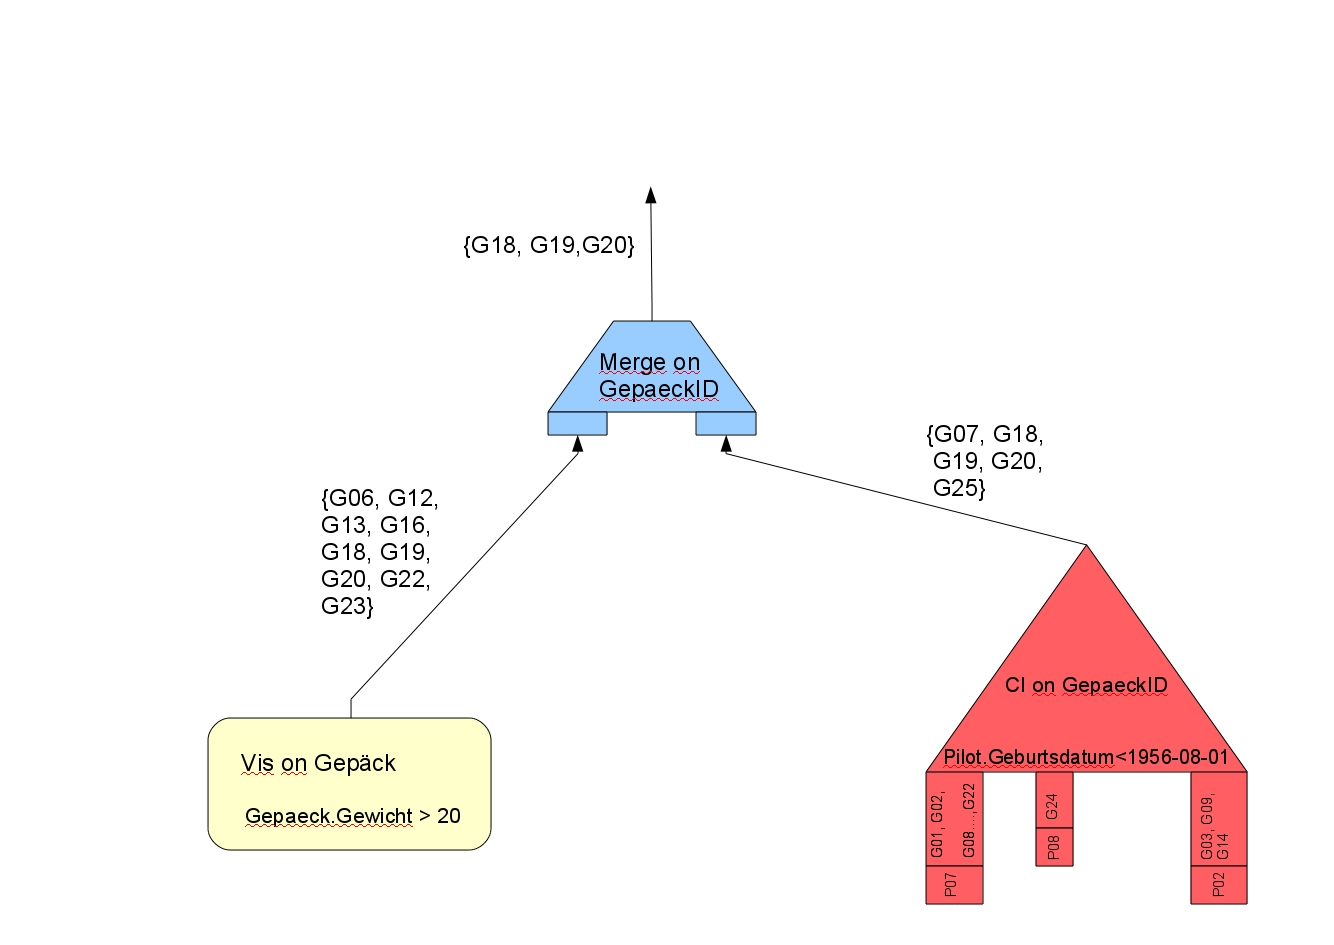
\includegraphics[width=1\linewidth]{img/Pre1}
  \caption{Teilergebnis Pre-Filtering 1}
  \label{fig:pre1}
\end{figure}

Von Piloten aus wird analog der Weg �ber Buchungen Buchungen beschritten. ``Climbing Index'': \{\{\}, \{B08, B11, B18, B19, B20, B21\}, \{\}, \{\}\}, Merge: \{B08, B11, B18, B19, B20, B21\}.

\begin{figure}[H]
  \centering
  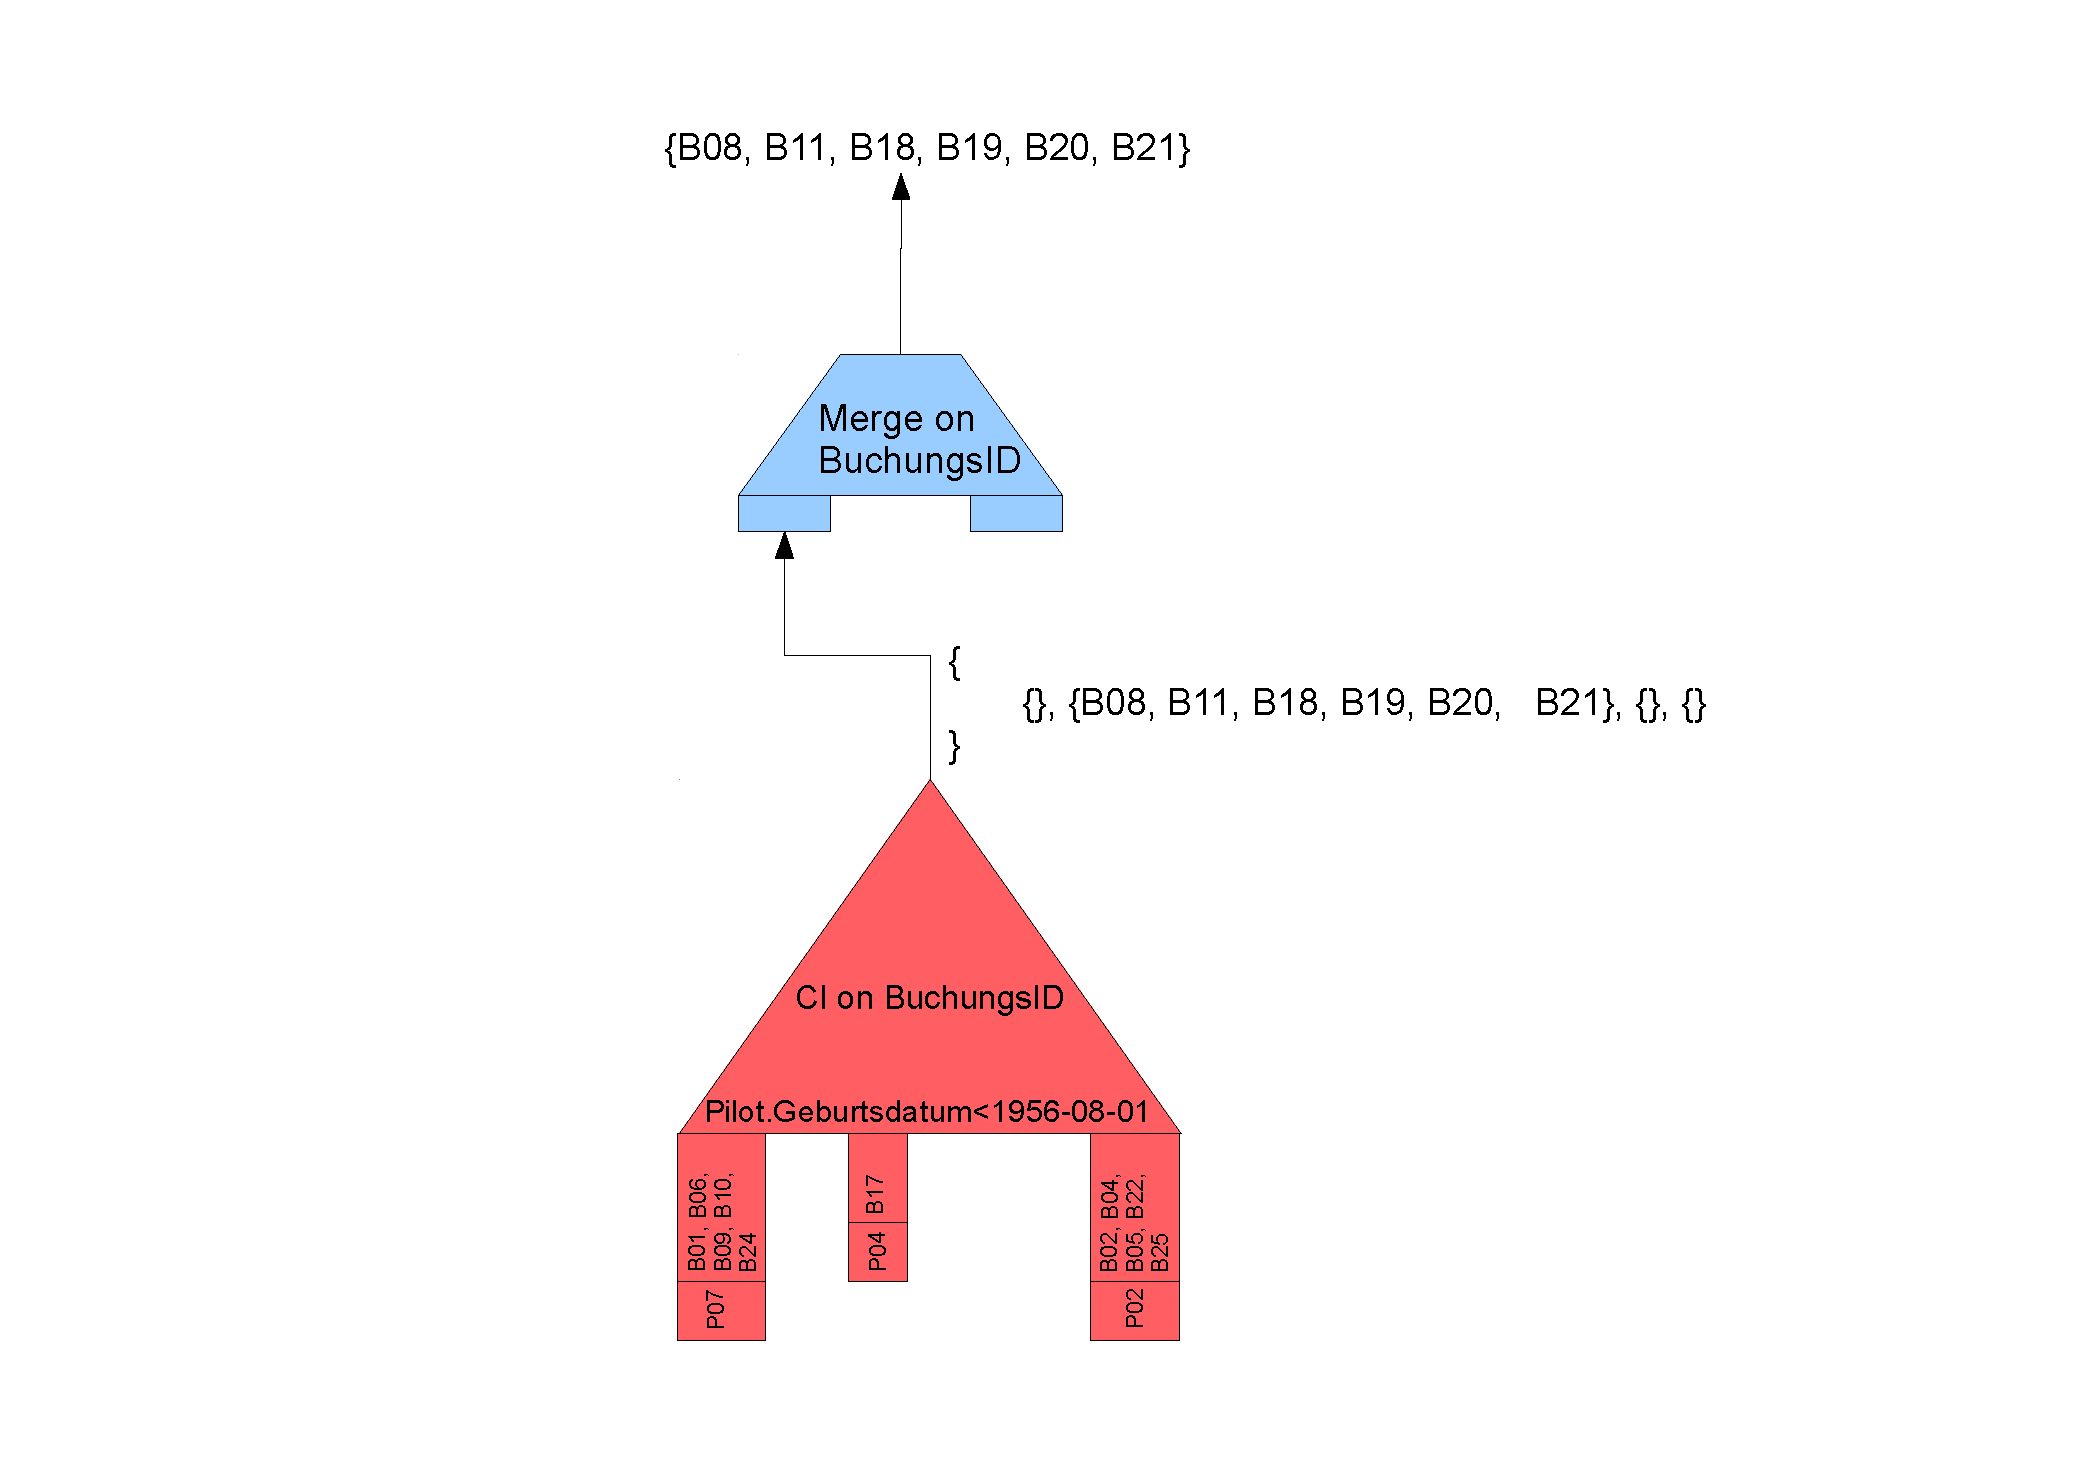
\includegraphics[width=1\linewidth]{img/Pre2.pdf}
  \caption{Teilergebnis Pre-Filtering 2}
  \label{fig:pre2}
\end{figure}

Unter Zuhilfenahme der entsprechenden ``Subtree Key Tables'' wird die Verbindung zur Tabelle \textit{Reisende} hergestellt: \{R07, R04, R04\} bzw. \{R07, R03, R13, R05, R04, R11\}. Mittels Merge wird der Durchschnitt beider Listen gebildet: \{R04, R07\}.

\begin{figure}[H]
  \centering
  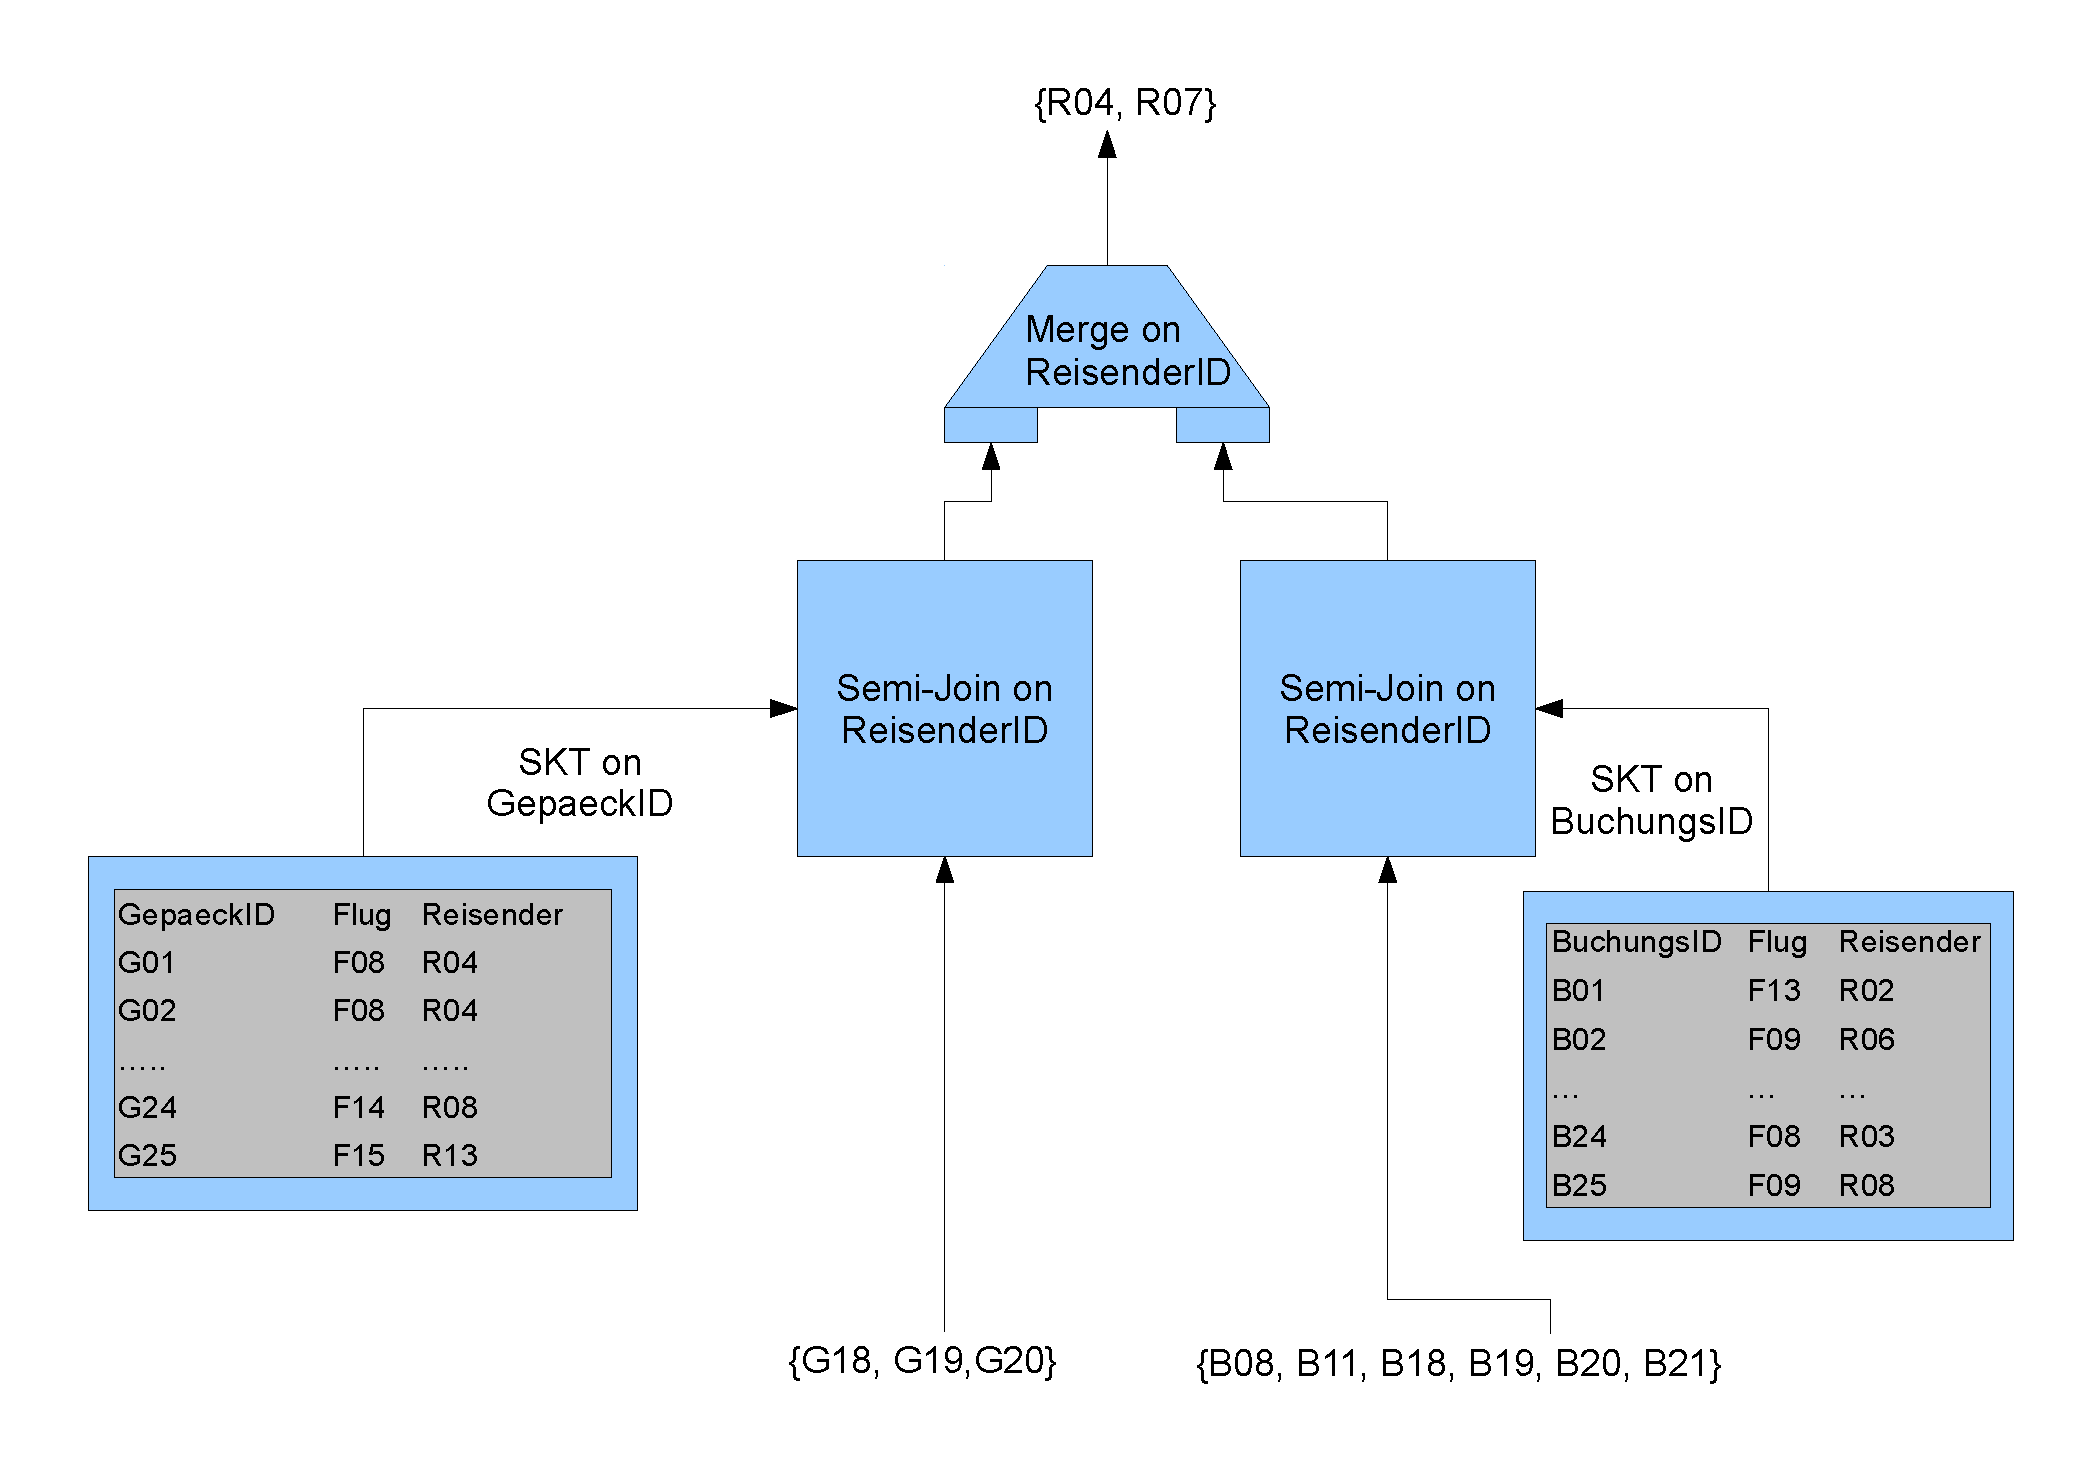
\includegraphics[width=1\linewidth]{img/Pre3.pdf}
  \caption{Teilergebnis Pre-Filtering 3}
  \label{fig:pre3}
\end{figure}

F�r die entstandene Liste wird ein Bloom-Filter erzeugt. Die noch ausstehende Selektion R.Geschlecht='M' wird vom unsicheren Ger�t ausgef�hrt und das Ergbnis mittels Bloom-Filter gefiltert.

\begin{figure}[H]
  \centering
  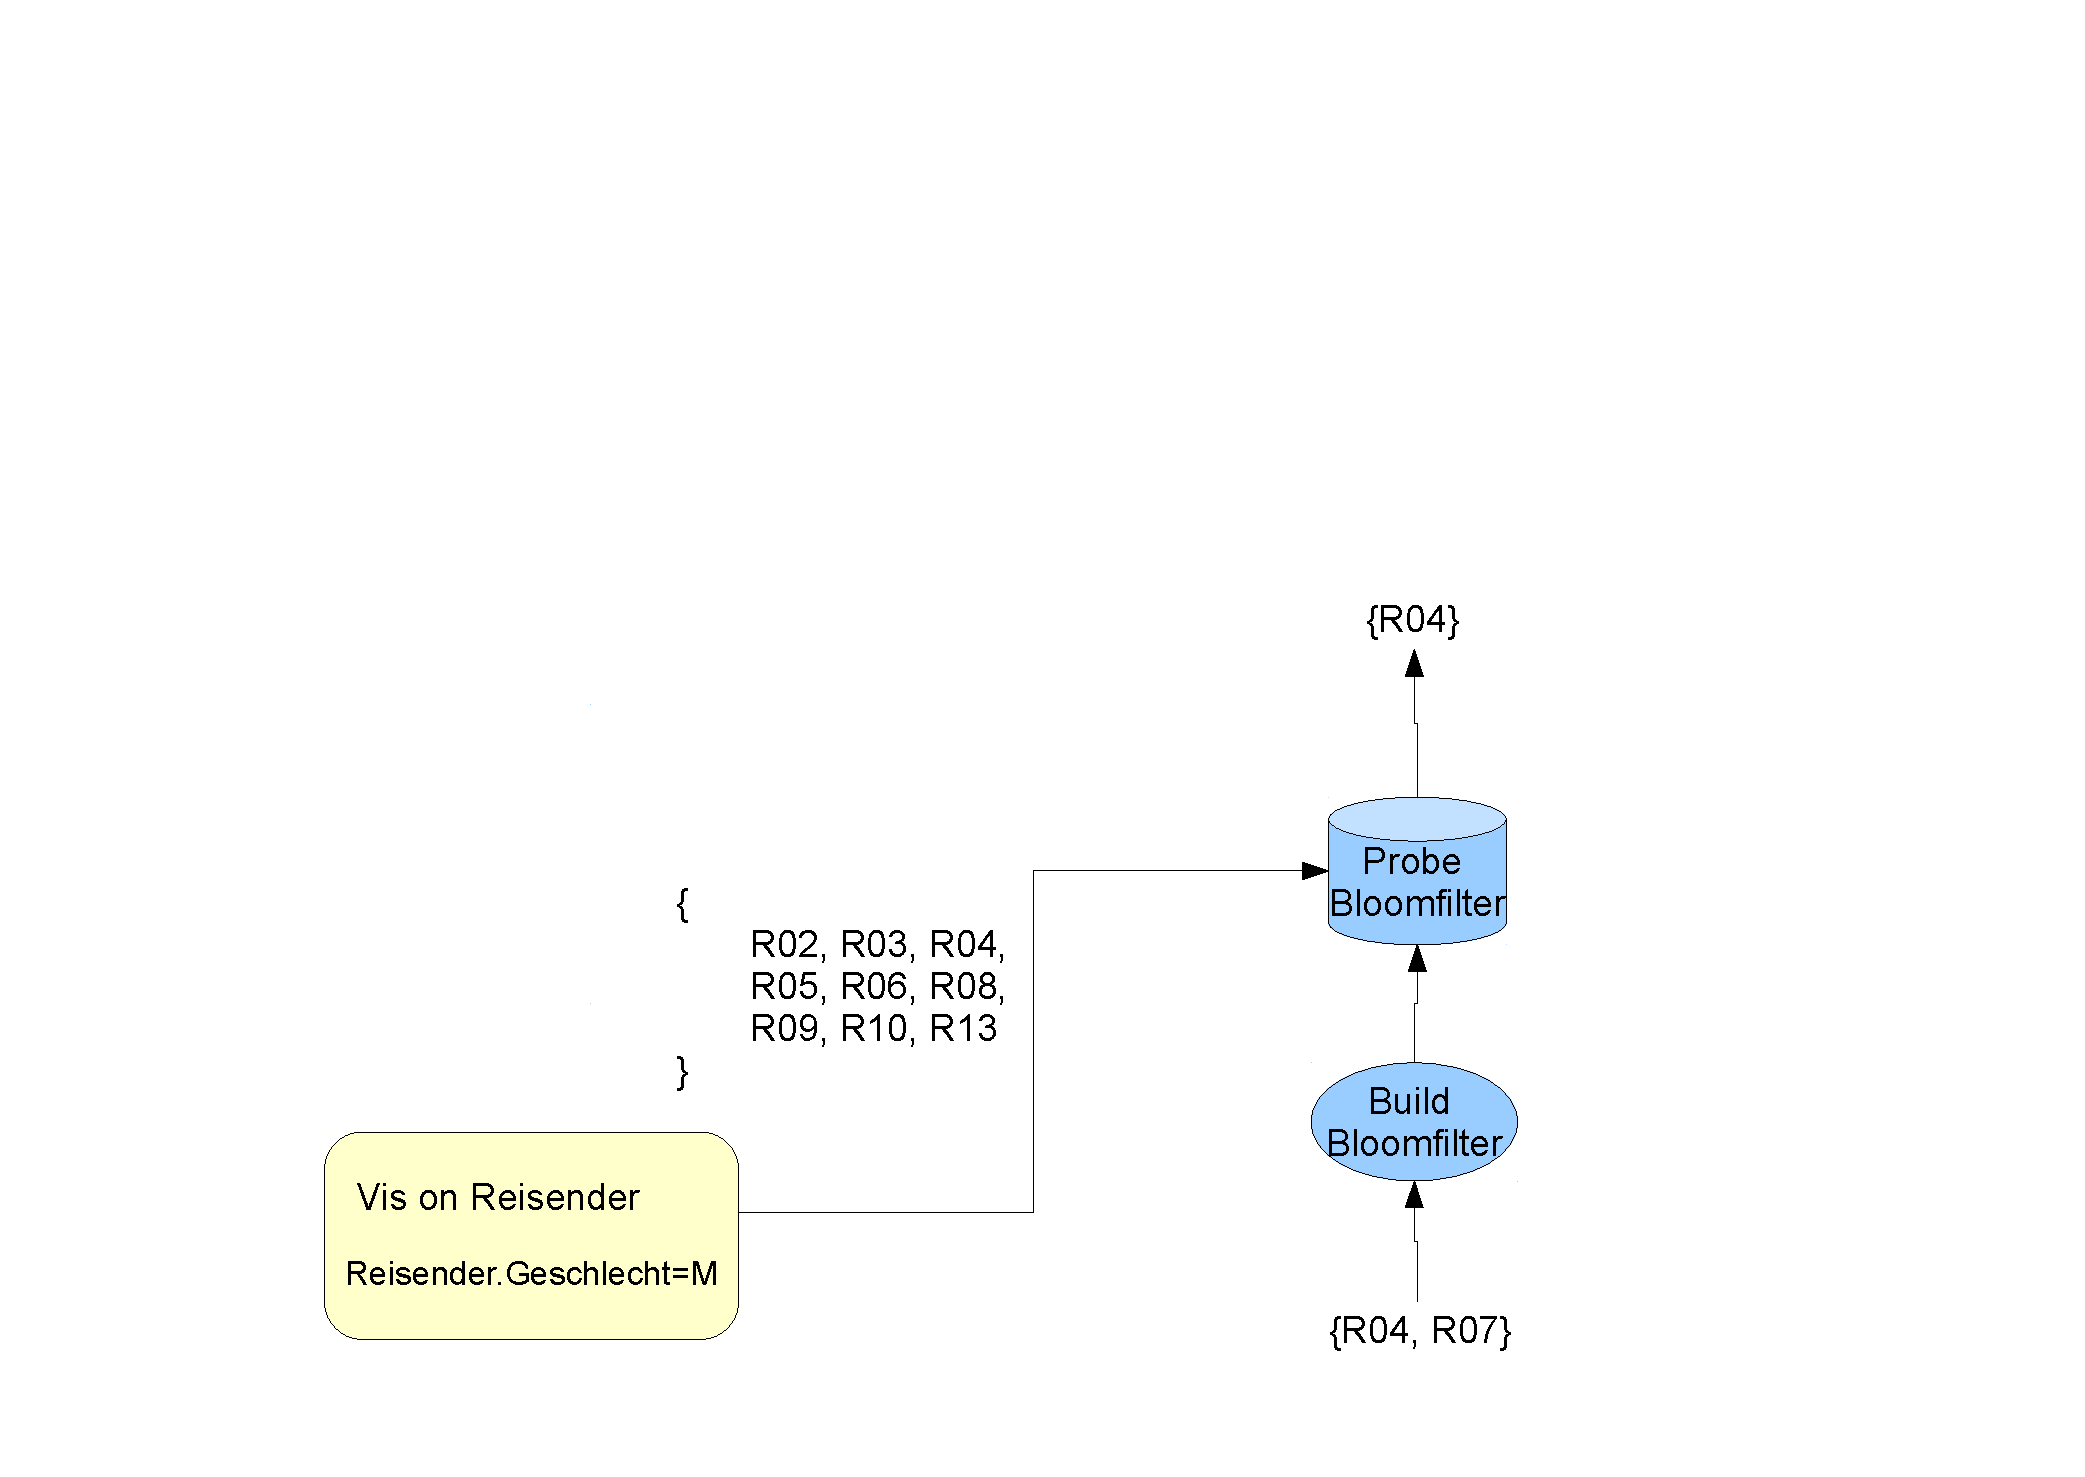
\includegraphics[width=1\linewidth]{img/Pre4.pdf}
  \caption{Teilergebnis Pre-Filtering 4}
  \label{fig:pre4}
\end{figure}

Mittels MJoin werden die noch verbleibenden Projektionen ausgef�hrt: \{$\langle$R04,Doru,Davidovici,Rom�nisch$\rangle$\}.

\begin{figure}[H]
  \centering
  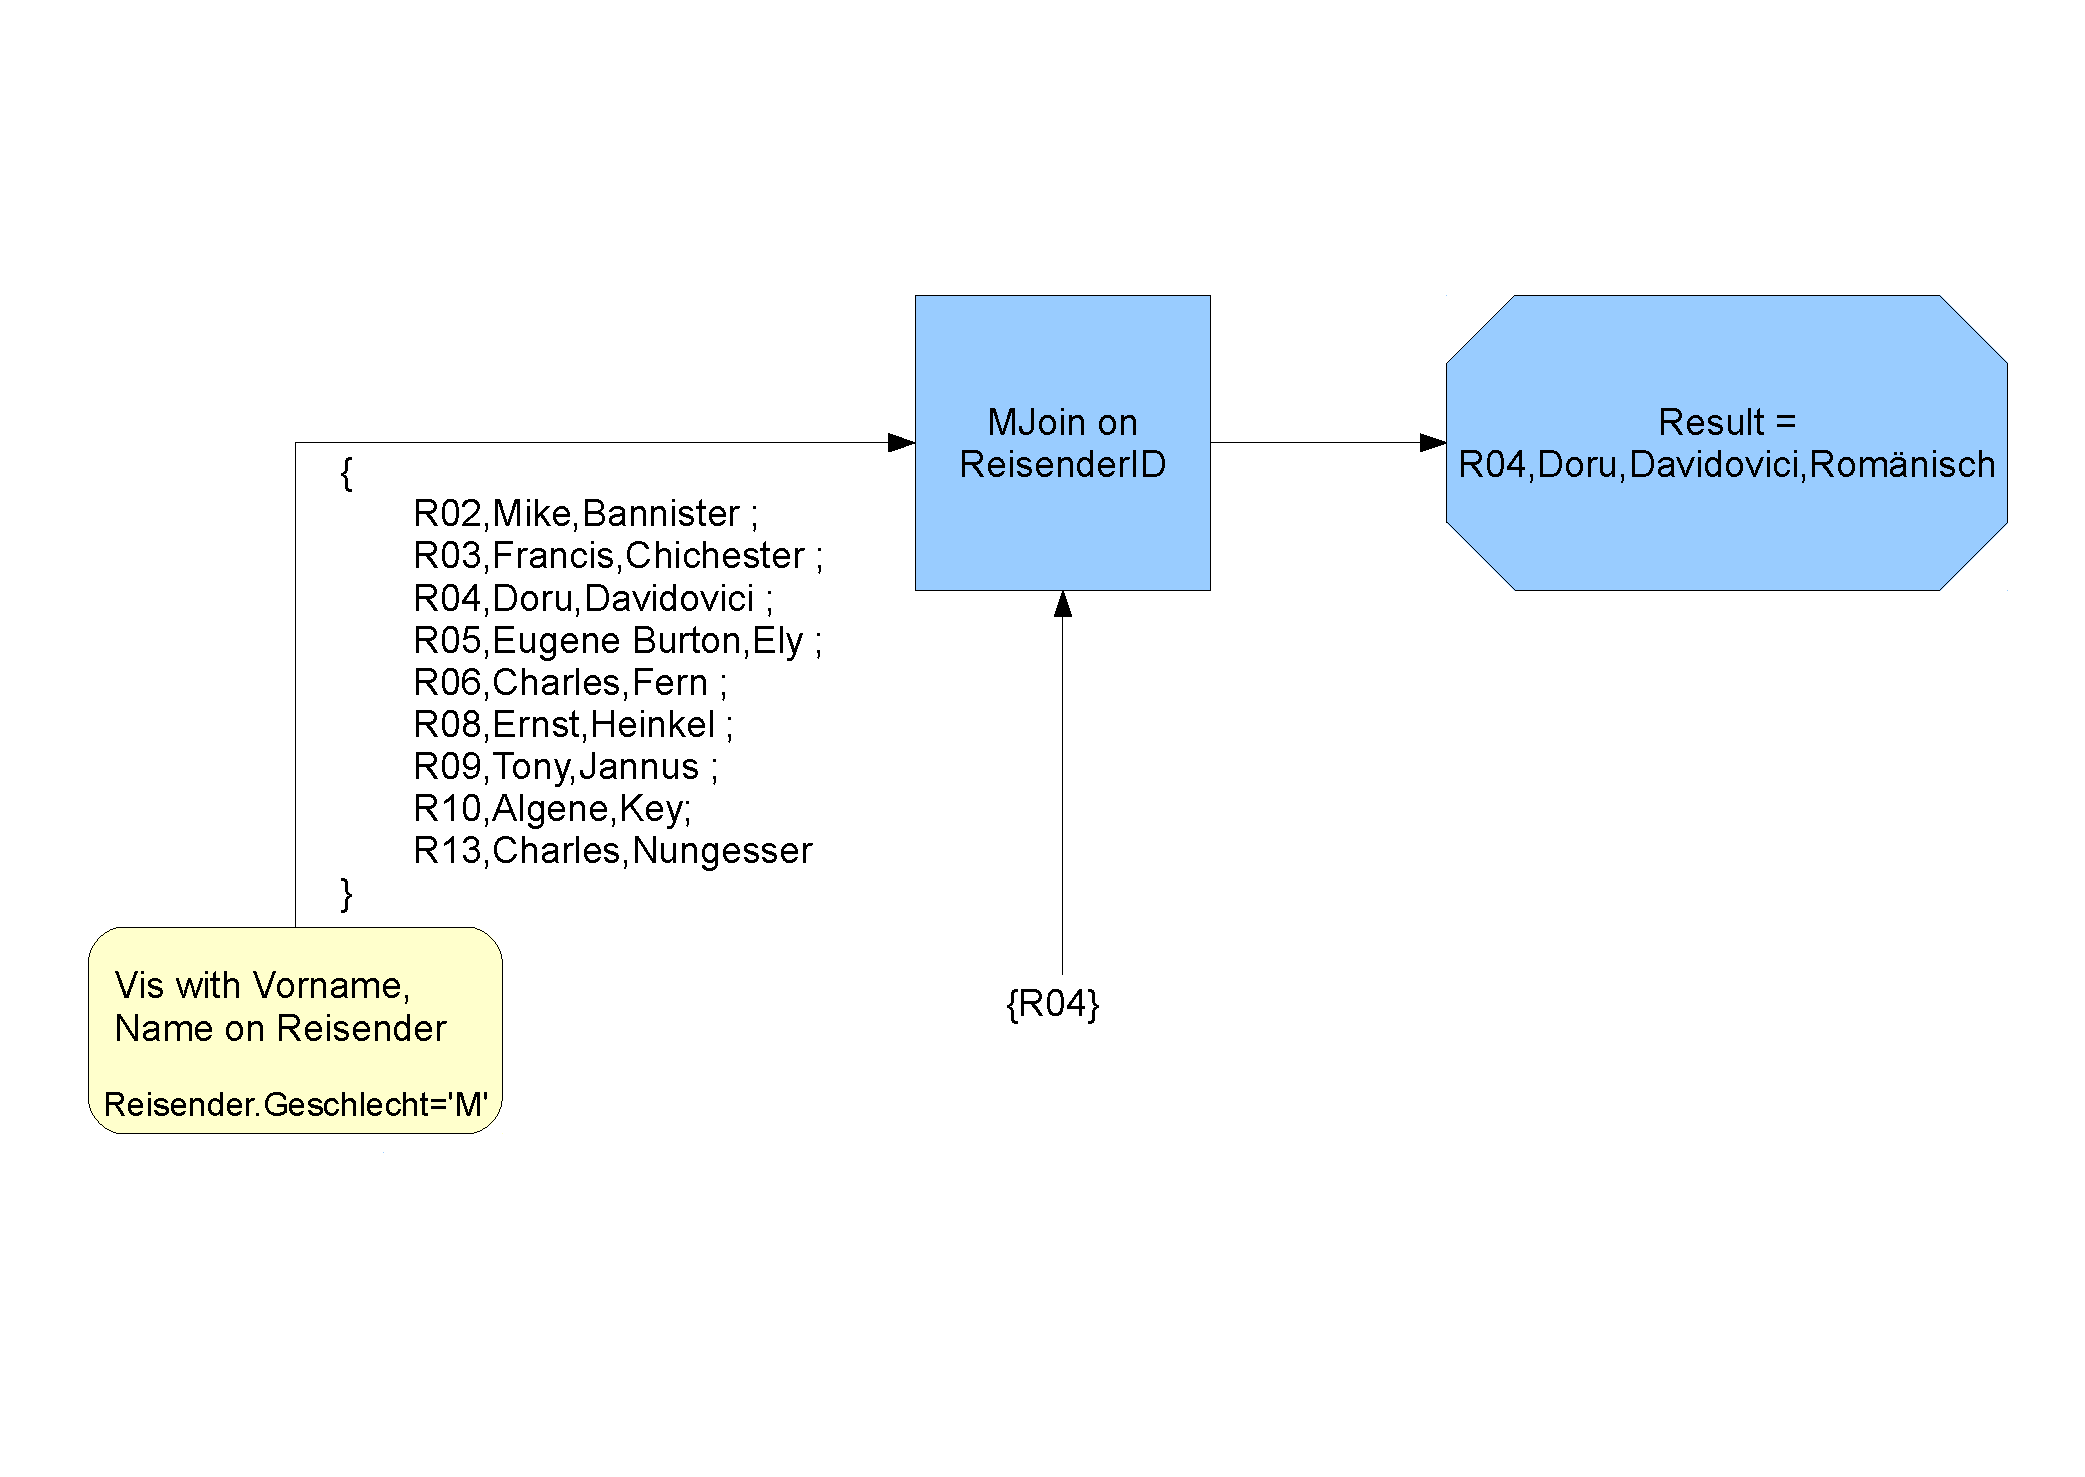
\includegraphics[width=1\linewidth]{img/Pre5.pdf}
  \caption{Teilergebnis Pre-Filtering 5}
  \label{fig:pre5}
\end{figure}

F�gt man die einzelnen Schritte zusammen entsteht folgender Ausf�hrungsplan f�r das Prefiltering:

\begin{figure}[H]
  \centering
  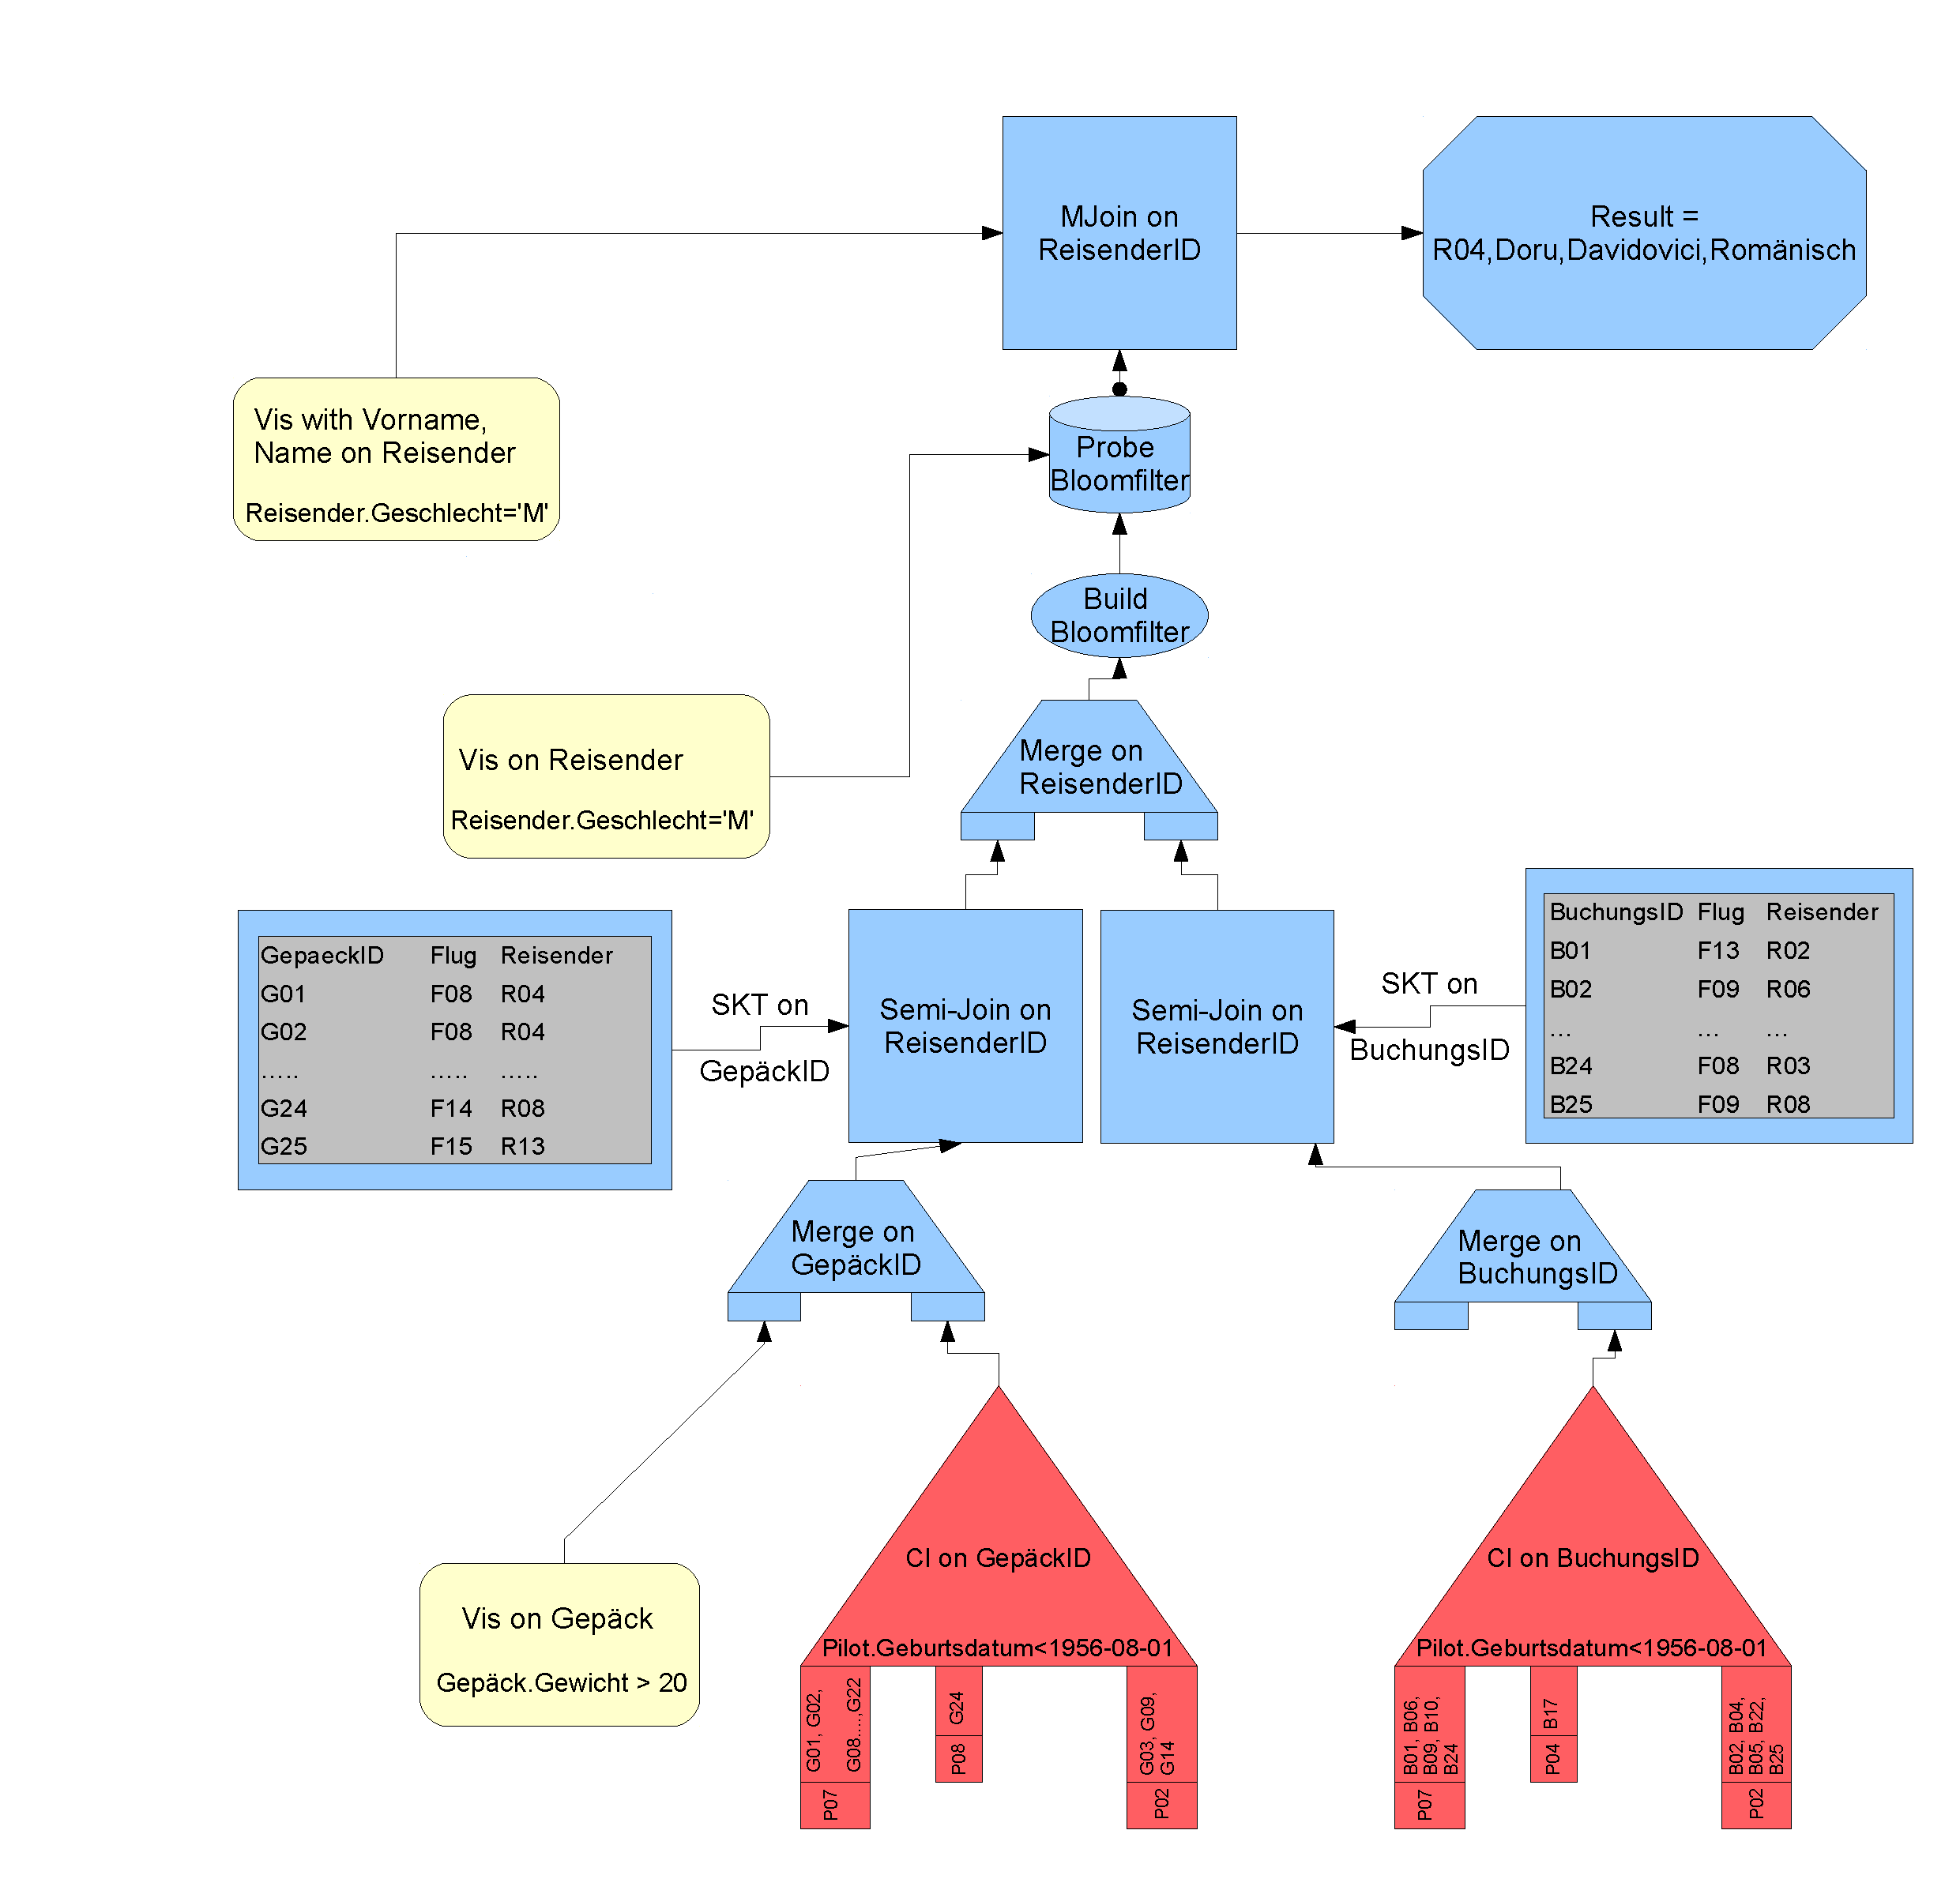
\includegraphics[width=1\linewidth]{img/Pre-Filtering.pdf}
  \caption{Pre-Filtering QEP}
  \label{fig:pre}
\end{figure}

\subsection{Pre-Filtering Funktionsaufrufe}
\begin{enumerate}[1]
\item Vis(Q,Gepaeck,G.GepaeckID) = \{G06, G12, G13, G16, G18, G19, G20, G22, G23\}
\item CI(P.Geburtsdatum,<1956-08-01,G.GepaeckID) = \{\{\}, \{G07, G18, G19, G20, G25\}, \{\}, \{\}\}
\item Merge(($\bigcup 2)\cap 1$) = \{G18, G19, G20\}
\item SJoin(3,$\text{SKT}_{\text{Gepaeck}}$,R.ReisenderID) = \{R07, R04, R04\}
\item CI(P.Geburtsdatum,<1956-08-01,B.BuchungsID) = \{\{\}, \{B08, B11, B18, B19, B20, B21\}, \{\}, \{\}\}
\item Merge($\bigcup 5$) = \{B08, B11, B18, B19, B20, B21\}
\item SJoin(6,$\text{SKT}_{\text{Buchungen}}$,R.ReisenderID) = \{R07, R03, R13, R05, R04, R11\}
\item Merge($4\cap 7$) = \{R04, R07\}
\item BuildBF(8) = BF
\item Vis(Q,Reisende,R.ReisenderID) = \{R02, R03, R04, R05, R06, R08, R09, R10, R13\}
\item ProbeBF(BF,10) = \{R04\}
\item Vis(Q,Reisende,$\langle$R.ReisenderID,R.Vorname,R.Name$\rangle$) = \{$\langle$R02,Mike,Bannister$\rangle$, \\
$\langle$R03,Francis,Chichester$\rangle$, $\langle$R04,Doru,Davidovici$\rangle$, $\langle$R05,Eugene Burton,Ely$\rangle$, $\langle$R06,Charles,Fern$\rangle$, $\langle$R08,Ernst,Heinkel$\rangle$, $\langle$R09,Tony,Jannus$\rangle$, $\langle$R10,Algene,Key$\rangle$, $\langle$R13,Charles,Nungesser$\rangle$\}
\item MJoin(12,11,$\langle$R.ReisenderID,R.Staatsbuergerschaft$\rangle$,8) = \{$\langle$R04,Doru,Davidovici,Rom�nisch$\rangle$\}
\end{enumerate}

Das Problem an dieser Strategie ist allerdings, dass bei zu geringer Selektivit�t der sichtbaren Selektionen zu wenige Tupel im Vorfeld aussortiert werden und somit ein gro�er Vorteil des Prefilterings verschwindet. Eine Alternative, die diesem Effekt entgegen wirkt ist das Postfiltering.

\section{Postfiltering}
Beim Postfiltering werden zuerst alle Selektionen ausgef�hrt und mittels Joins zusammengefasst, die auf den sicheren Bereich zugreifen. Erst danach werden unter Verwendung von Bloom-Filtern die Selektionen des unsicheren Bereiches hinzugef�gt.

F�r unser Beispiel hei�t dies, dass zuerst die Selektion auf dem Geburtsdatum des Piloten ausgef�hrt wird. Es wird der ``Climbing Index'' verwendet um \textit{GepackIDs} zu erhalten: \{\{\}, \{G07, G18, G19, G20, G25\}, \{\}, \{\}\}.

\begin{figure}[H]
  \centering
  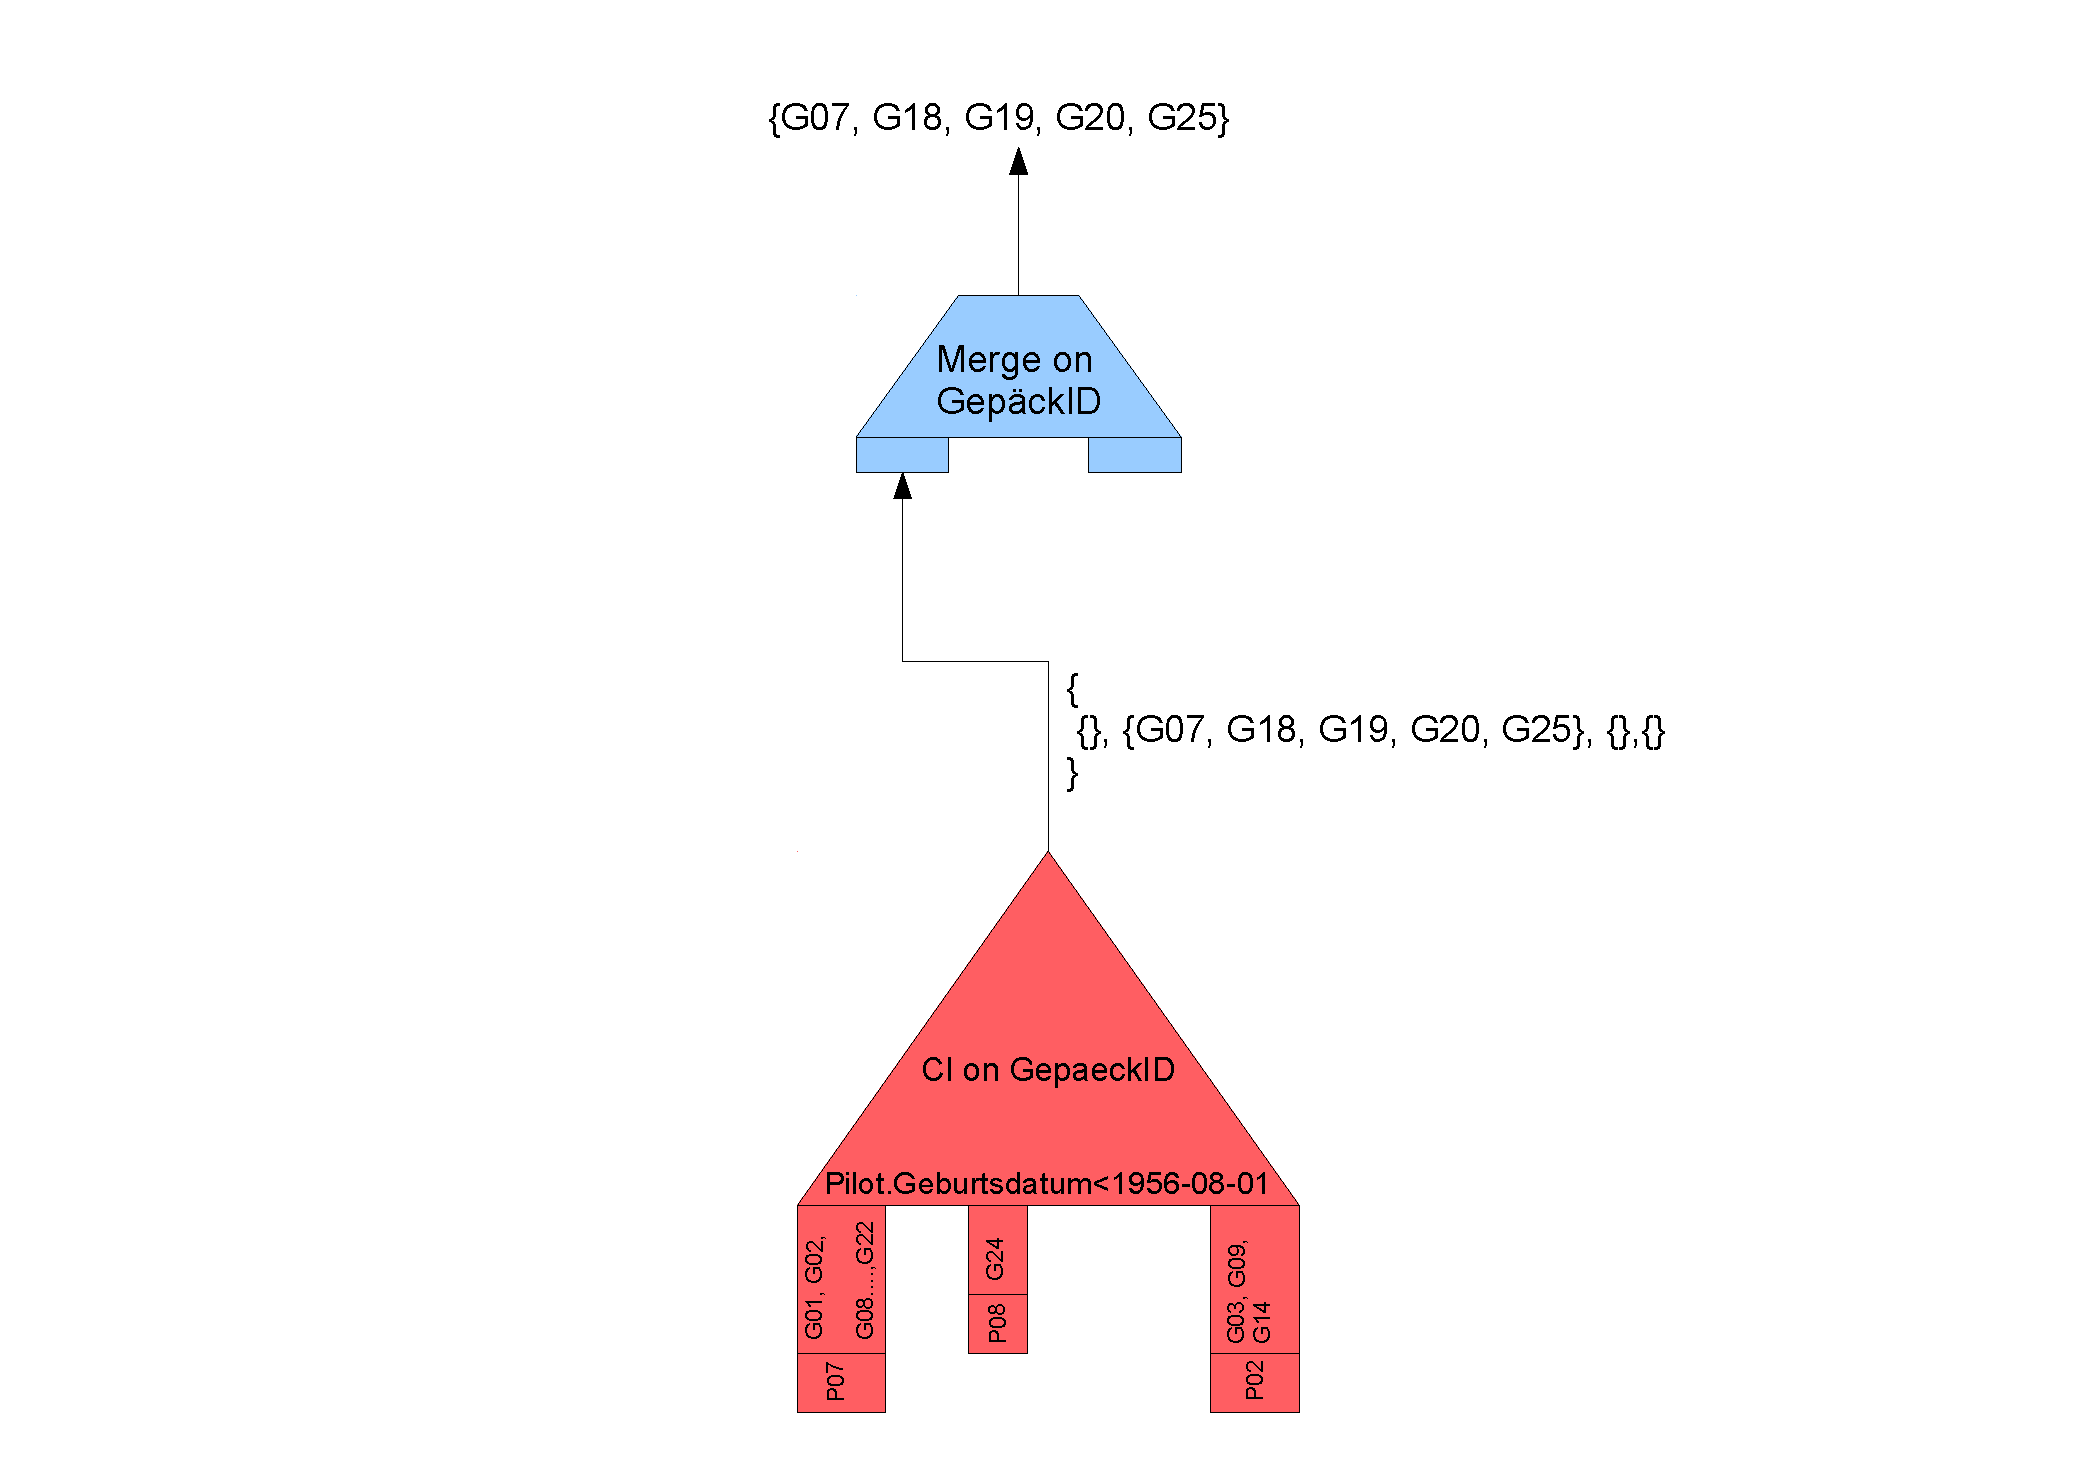
\includegraphics[width=1\linewidth]{img/Post1.pdf}
  \caption{Teilergebnis Post-Filtering 1}
  \label{fig:post1}
\end{figure}

Es wird ein ``Subtree Key Table'' verwendet, um passende \textit{ReisndeIDs} zu berechnen: \{$\langle$G07,R11$\rangle$, $\langle$G18,R07$\rangle$, $\langle$G19,R04$\rangle$, $\langle$G20,R04$\rangle$, $\langle$G22,R02$\rangle$, $\langle$G23,R01$\rangle$\}

\begin{figure}[H]
  \centering
  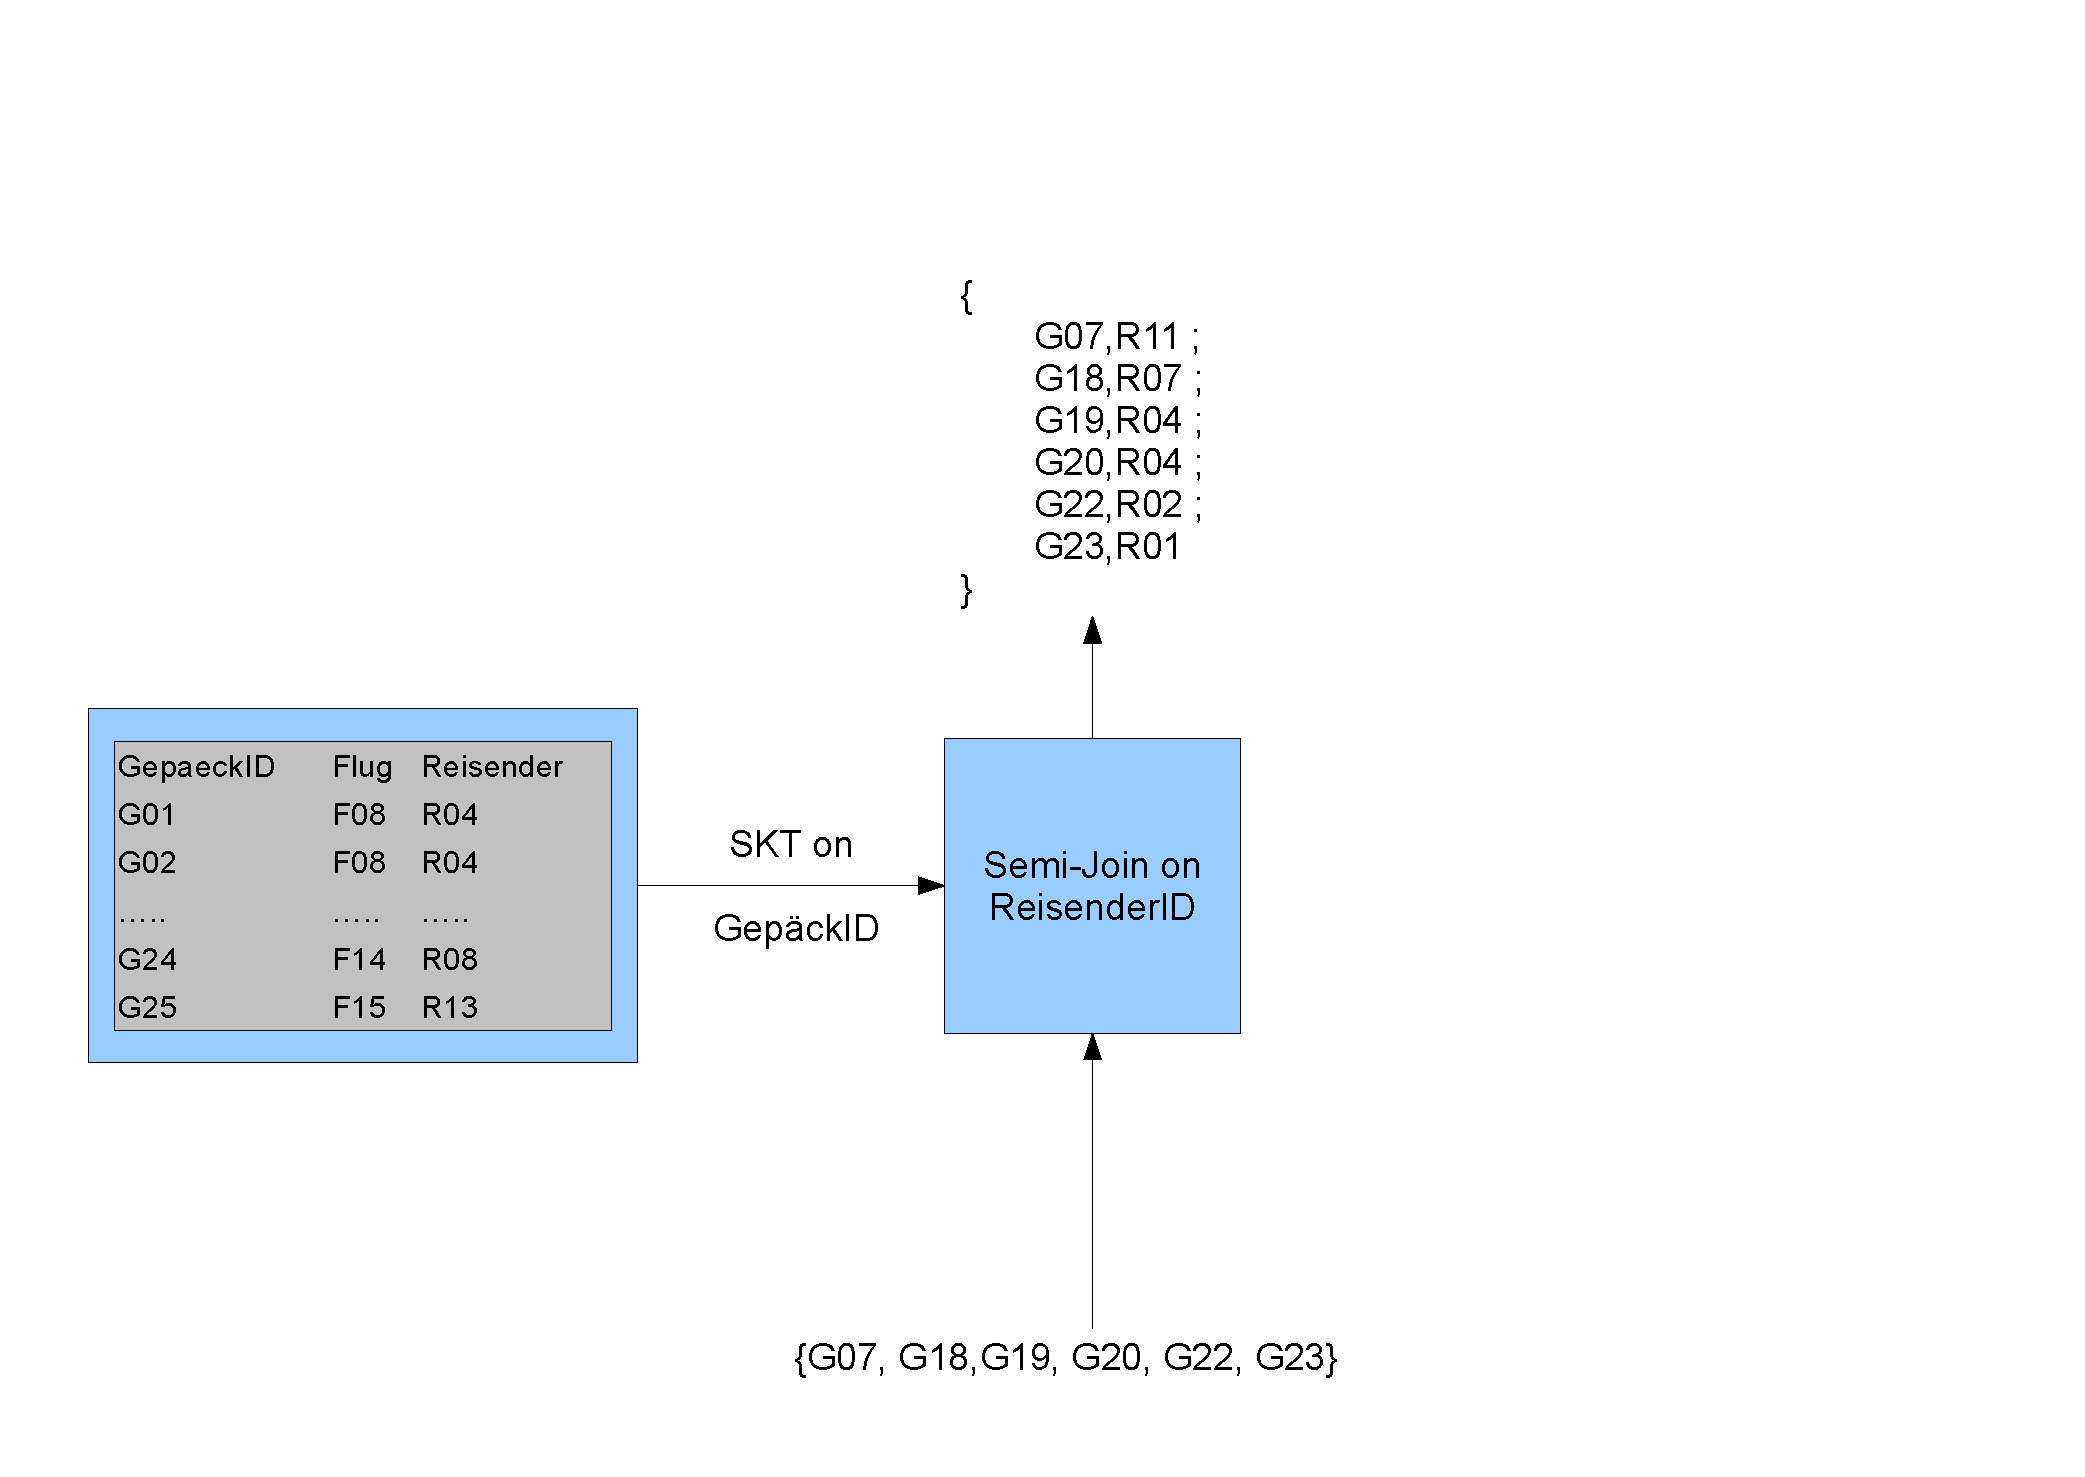
\includegraphics[width=1\textwidth]{img/Post2.pdf}
  \caption{Teilergebnis Post-Filtering 2}
  \label{fig:post2}
\end{figure}

Das unsichere Ger�t liefert die Gepc�kst�cke, die schwerer als 20 Kilogramm sind. Es wir dein Bloom-Filter erzeugt und auf das vorhandene Zwischenergebnis angewendet: \{$\langle$G07,R11$\rangle$, $\langle$G18,R07$\rangle$, $\langle$G19,R04$\rangle$, $\langle$G20,R04$\rangle$, $\langle$G22,R02$\rangle$, $\langle$G23,R01$\rangle$\}. Da die \textit{GepaeckIDs} nicht mehr ben�tigt werden, werden nur die \textit{ReisendeIDs} aufgehoben: \{R07, R04, R04, R02, R01\}

\begin{figure}[H]
  \centering
  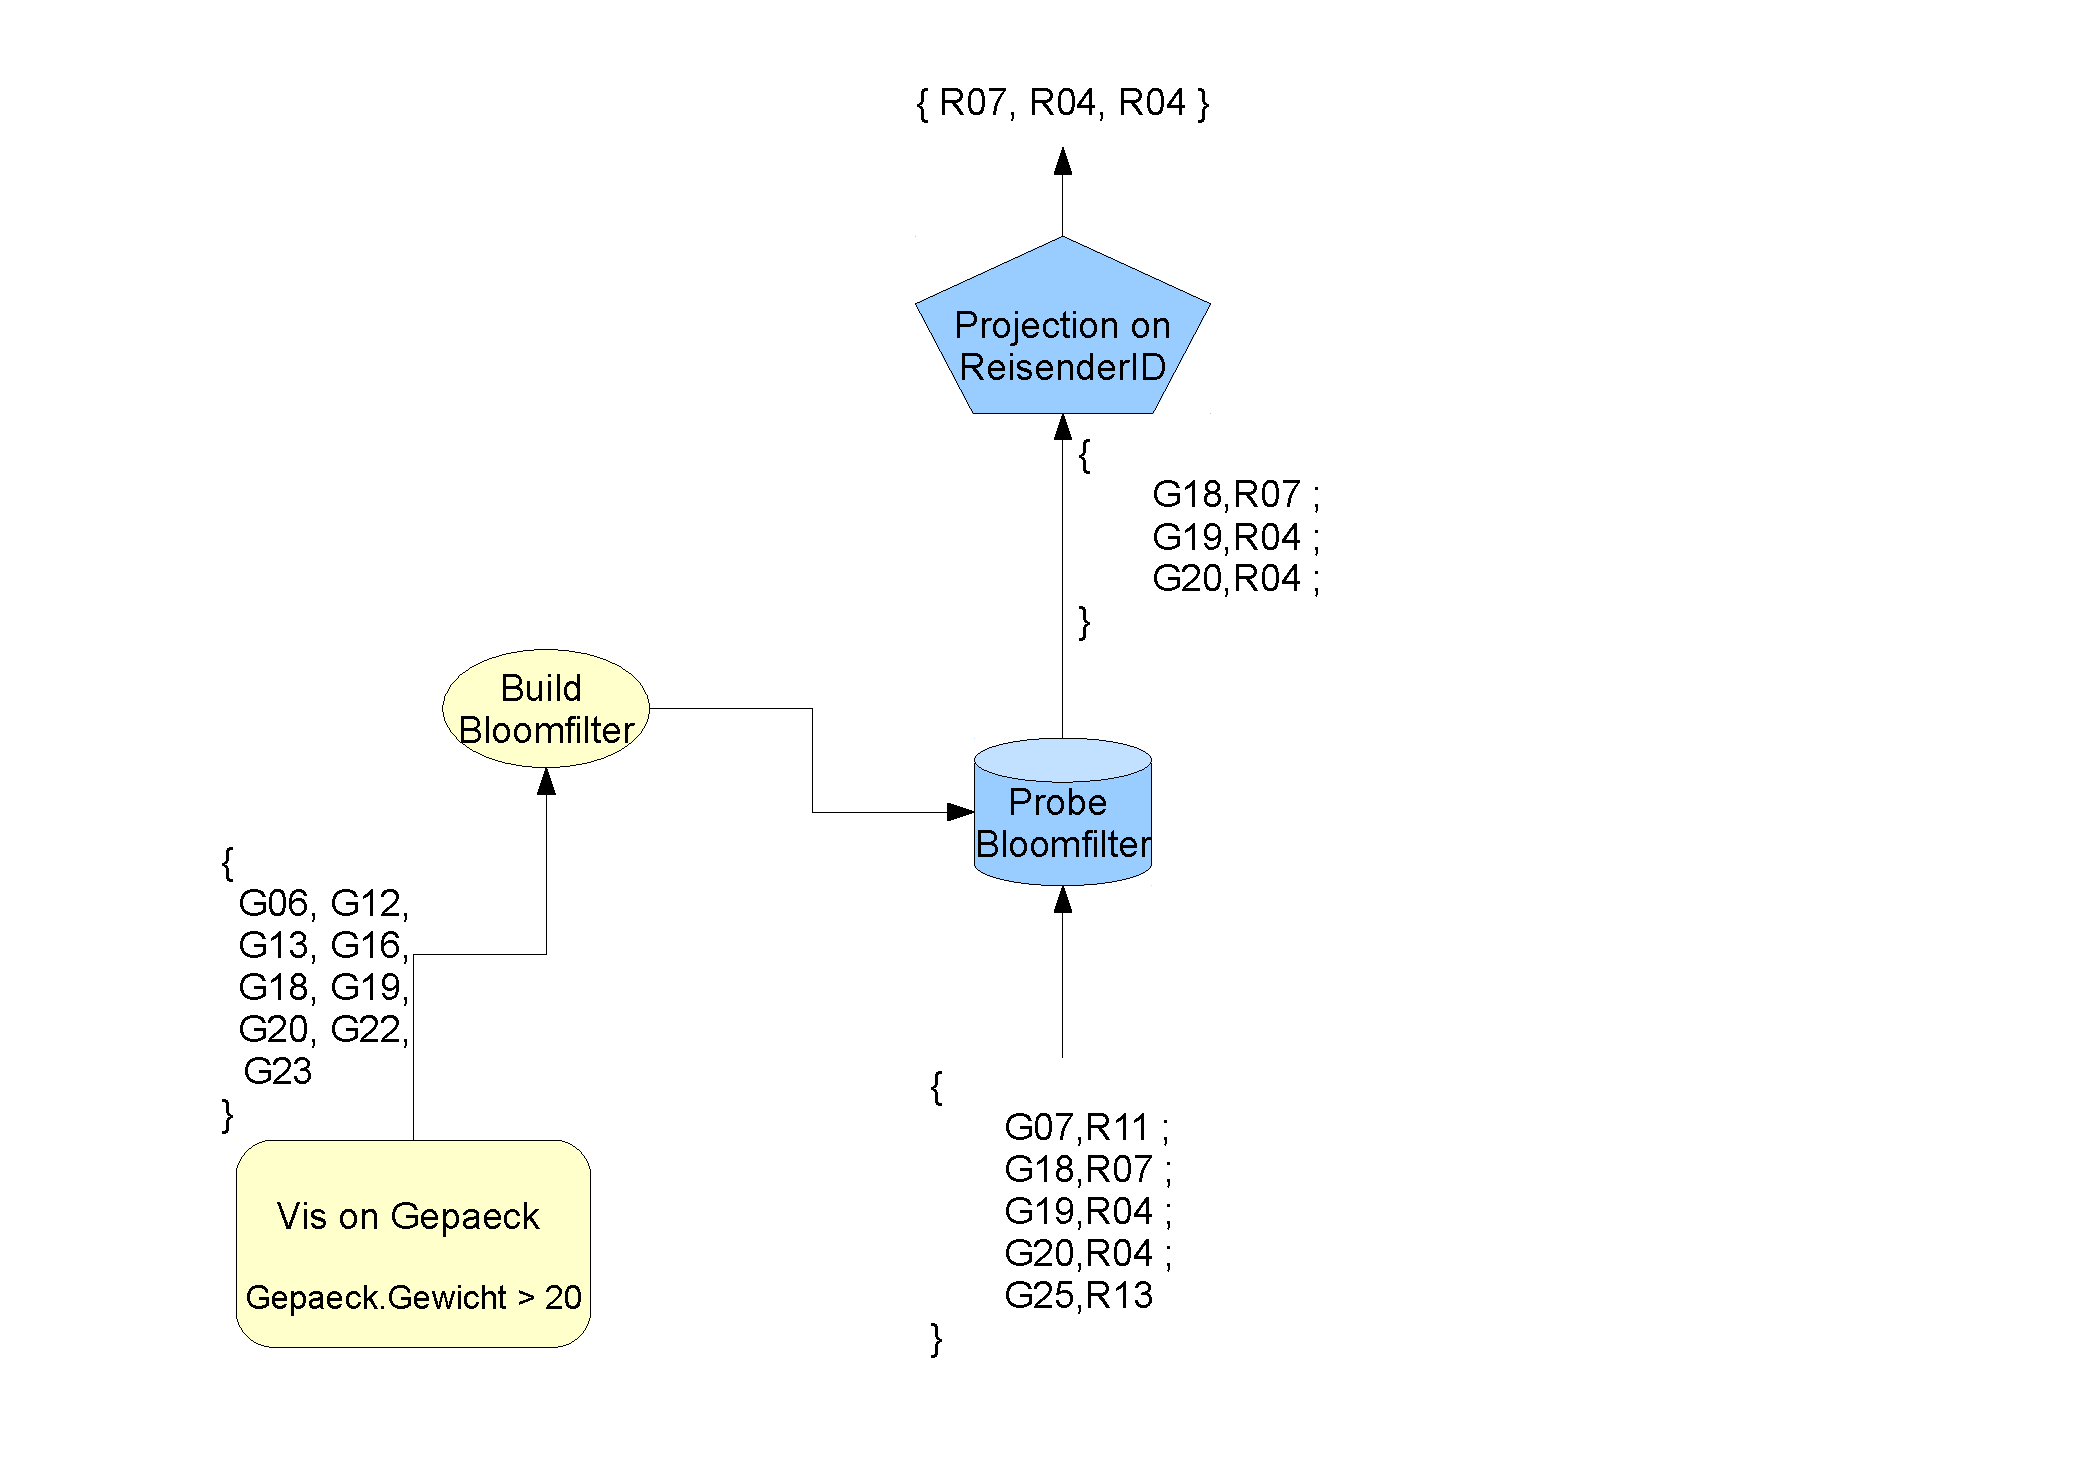
\includegraphics[width=1\textwidth]{img/Post3.pdf}
  \caption{Teilergebnis Post-Filtering 3}
  \label{fig:post3}
\end{figure}

Mittels ``Climbing Index'' ist der Schritt von \textit{Pilot.Geburtsdatum} auf \textit{BuchungsID} m�glich: \{\{\}, \{B08, B11, B18, B19, B20, B21\}, \{\}, \{\}\}. Durch Verwendung von Merge und eines ``Subtree Key Tables'' wird eine Liste von \textit{ReisendeIDs} berechnet: \{R07, R03, R13, R05, R04, R11\}.

\begin{figure}[H]
  \centering
  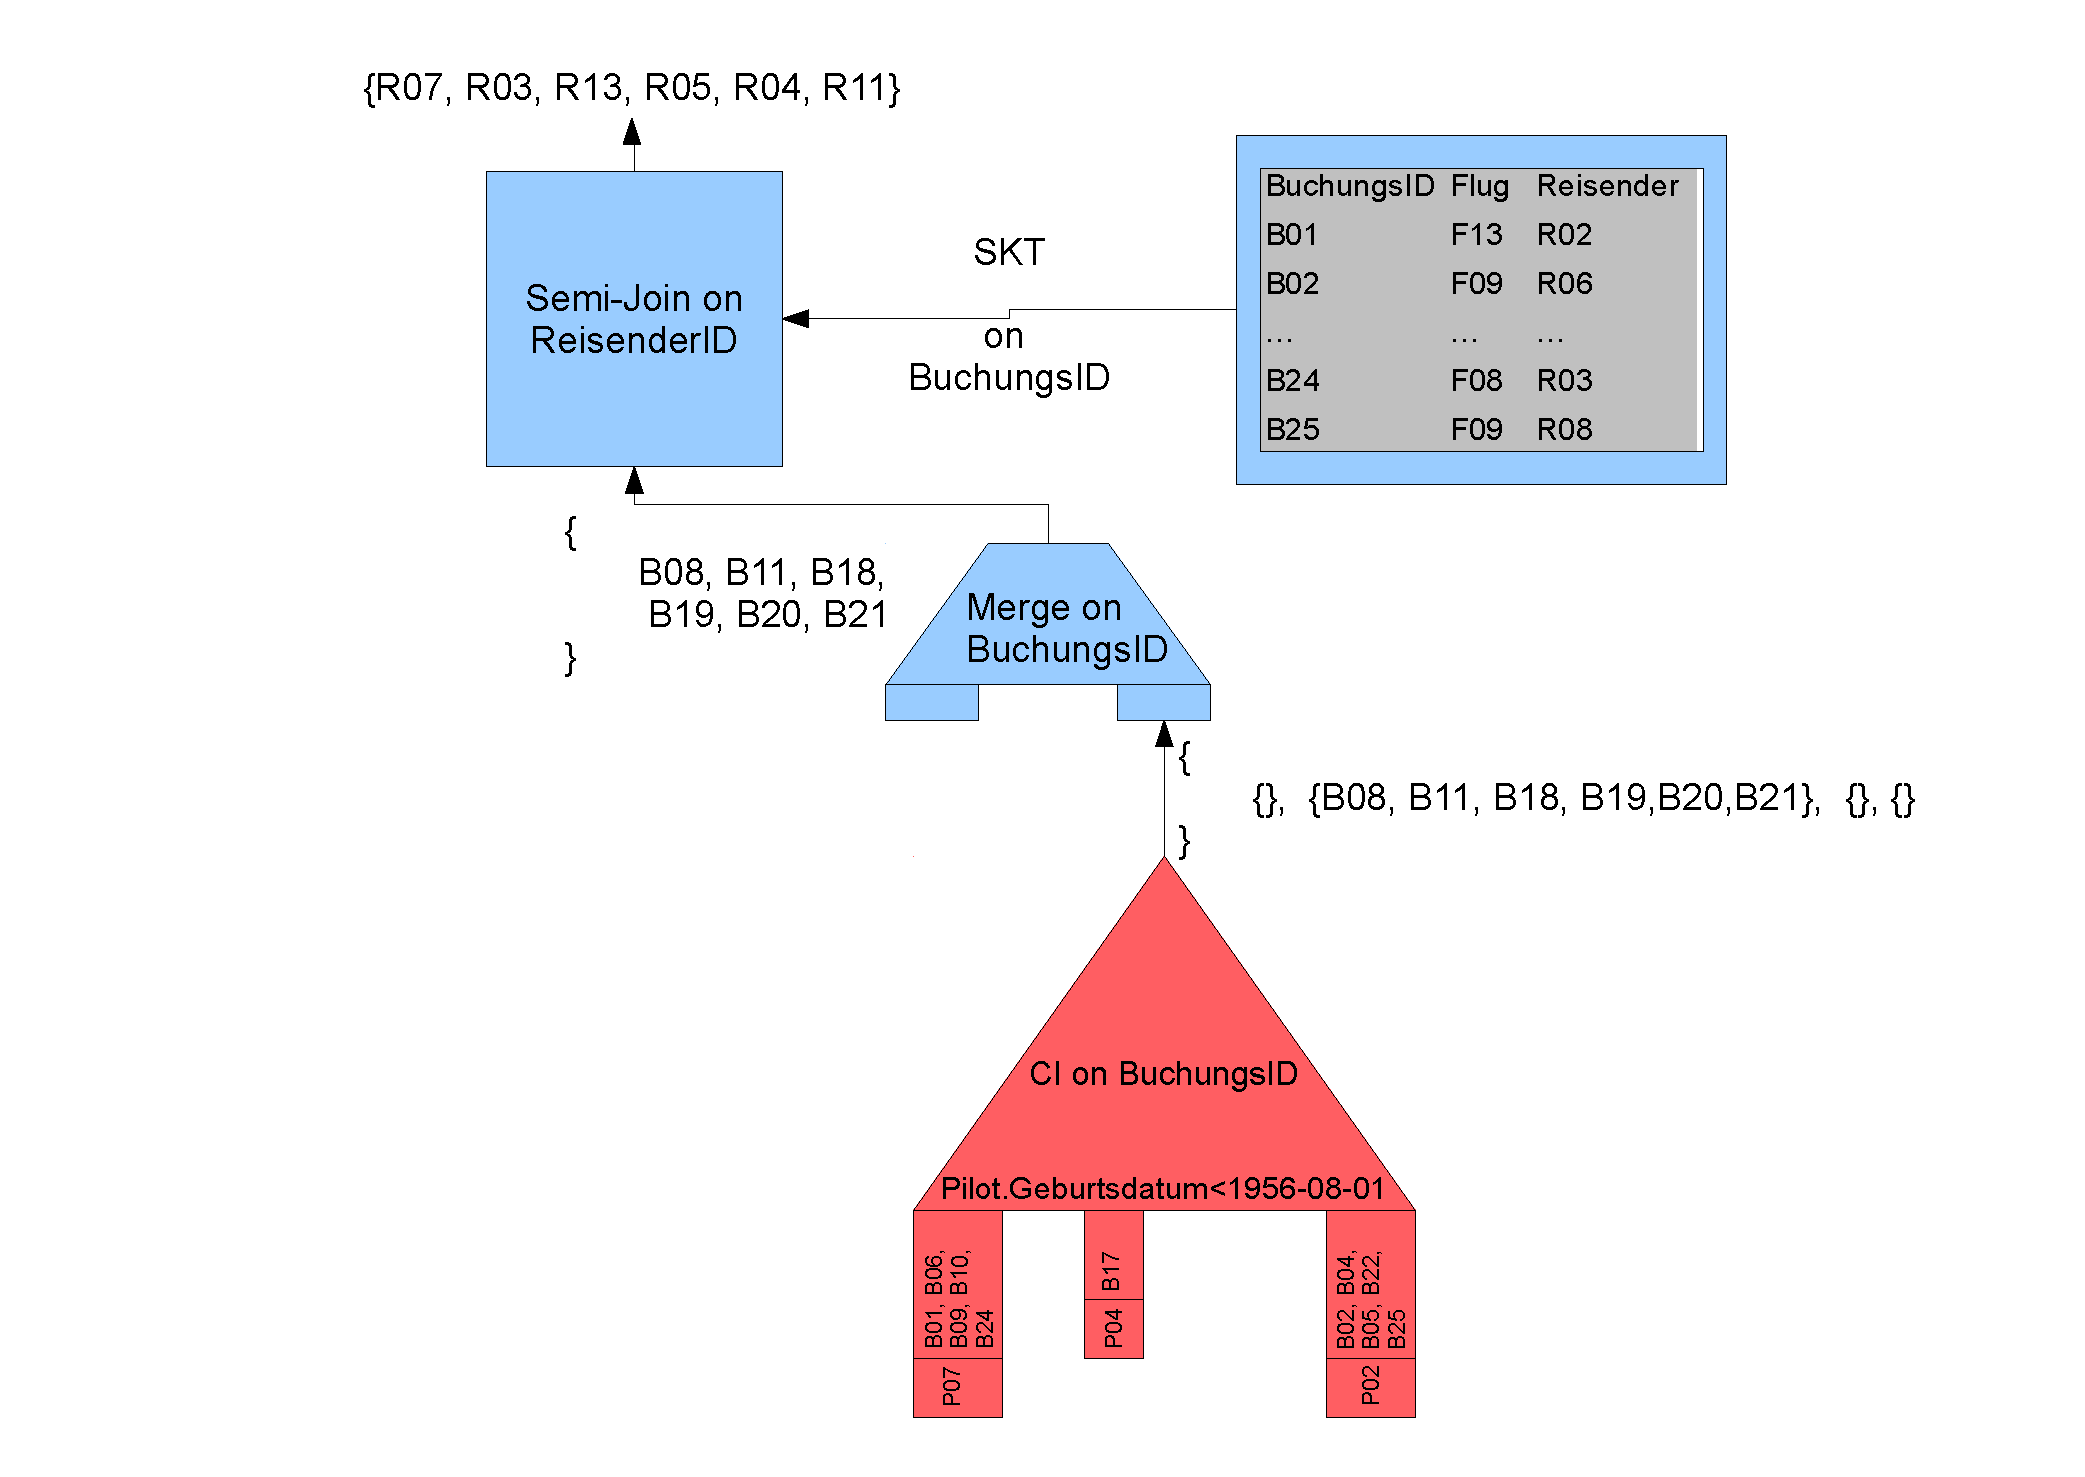
\includegraphics[width=1\textwidth]{img/Post4.pdf}
  \caption{Teilergebnis Post-Filtering 4}
  \label{fig:post4}
\end{figure}

Aus dem Durchschnitt beider Lsiten von \textit{ReisendeIDs} wird ein Bloom-Filter erzeugt. Dieser wird auf das �bermittelte Zwischenergebnis des unsicheren Ger�ts (Reisender.Geschlecht='M') angewendet. Durch Verwendung des MJoin-Operators wird das Ergebnis erzeugt: \{$\langle$R04,Doru,Davidovici,Rom�nisch$\rangle$\}.

\begin{figure}[H]
  \centering
  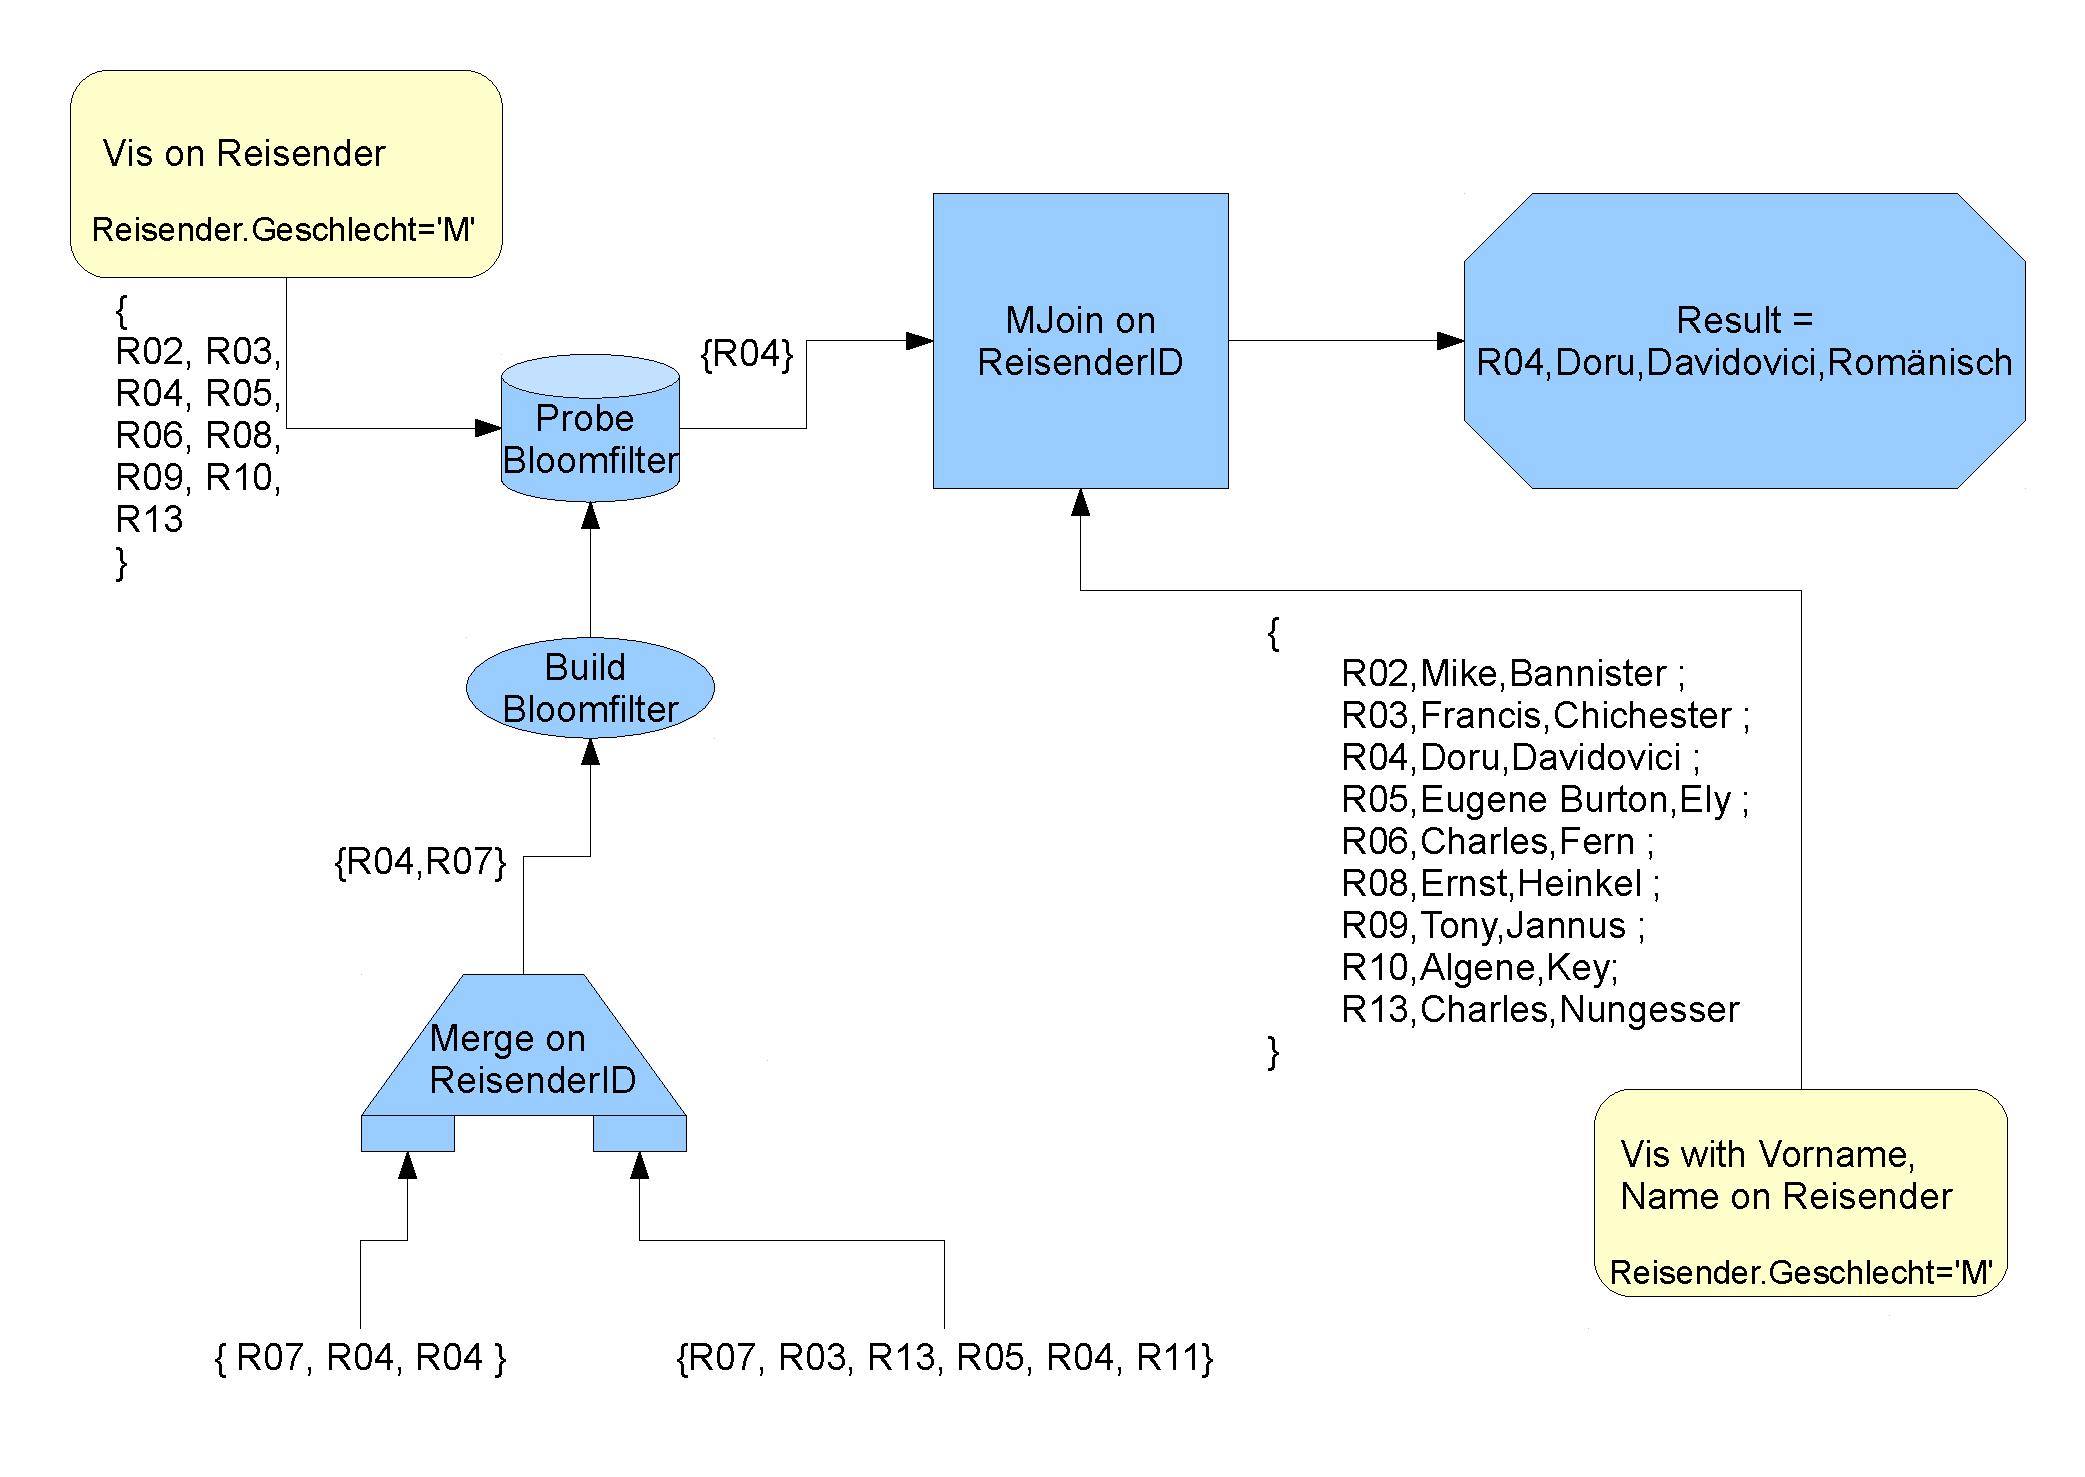
\includegraphics[width=1\textwidth]{img/Post5.pdf}
  \caption{Teilergebnis Post-Filtering 5}
  \label{fig:post5}
\end{figure}

F�gt man alle Teile zusammen erh�lt man den kompletten Ablaufplan f�r unsere Anfrage.

\begin{figure}[H]
  \centering
  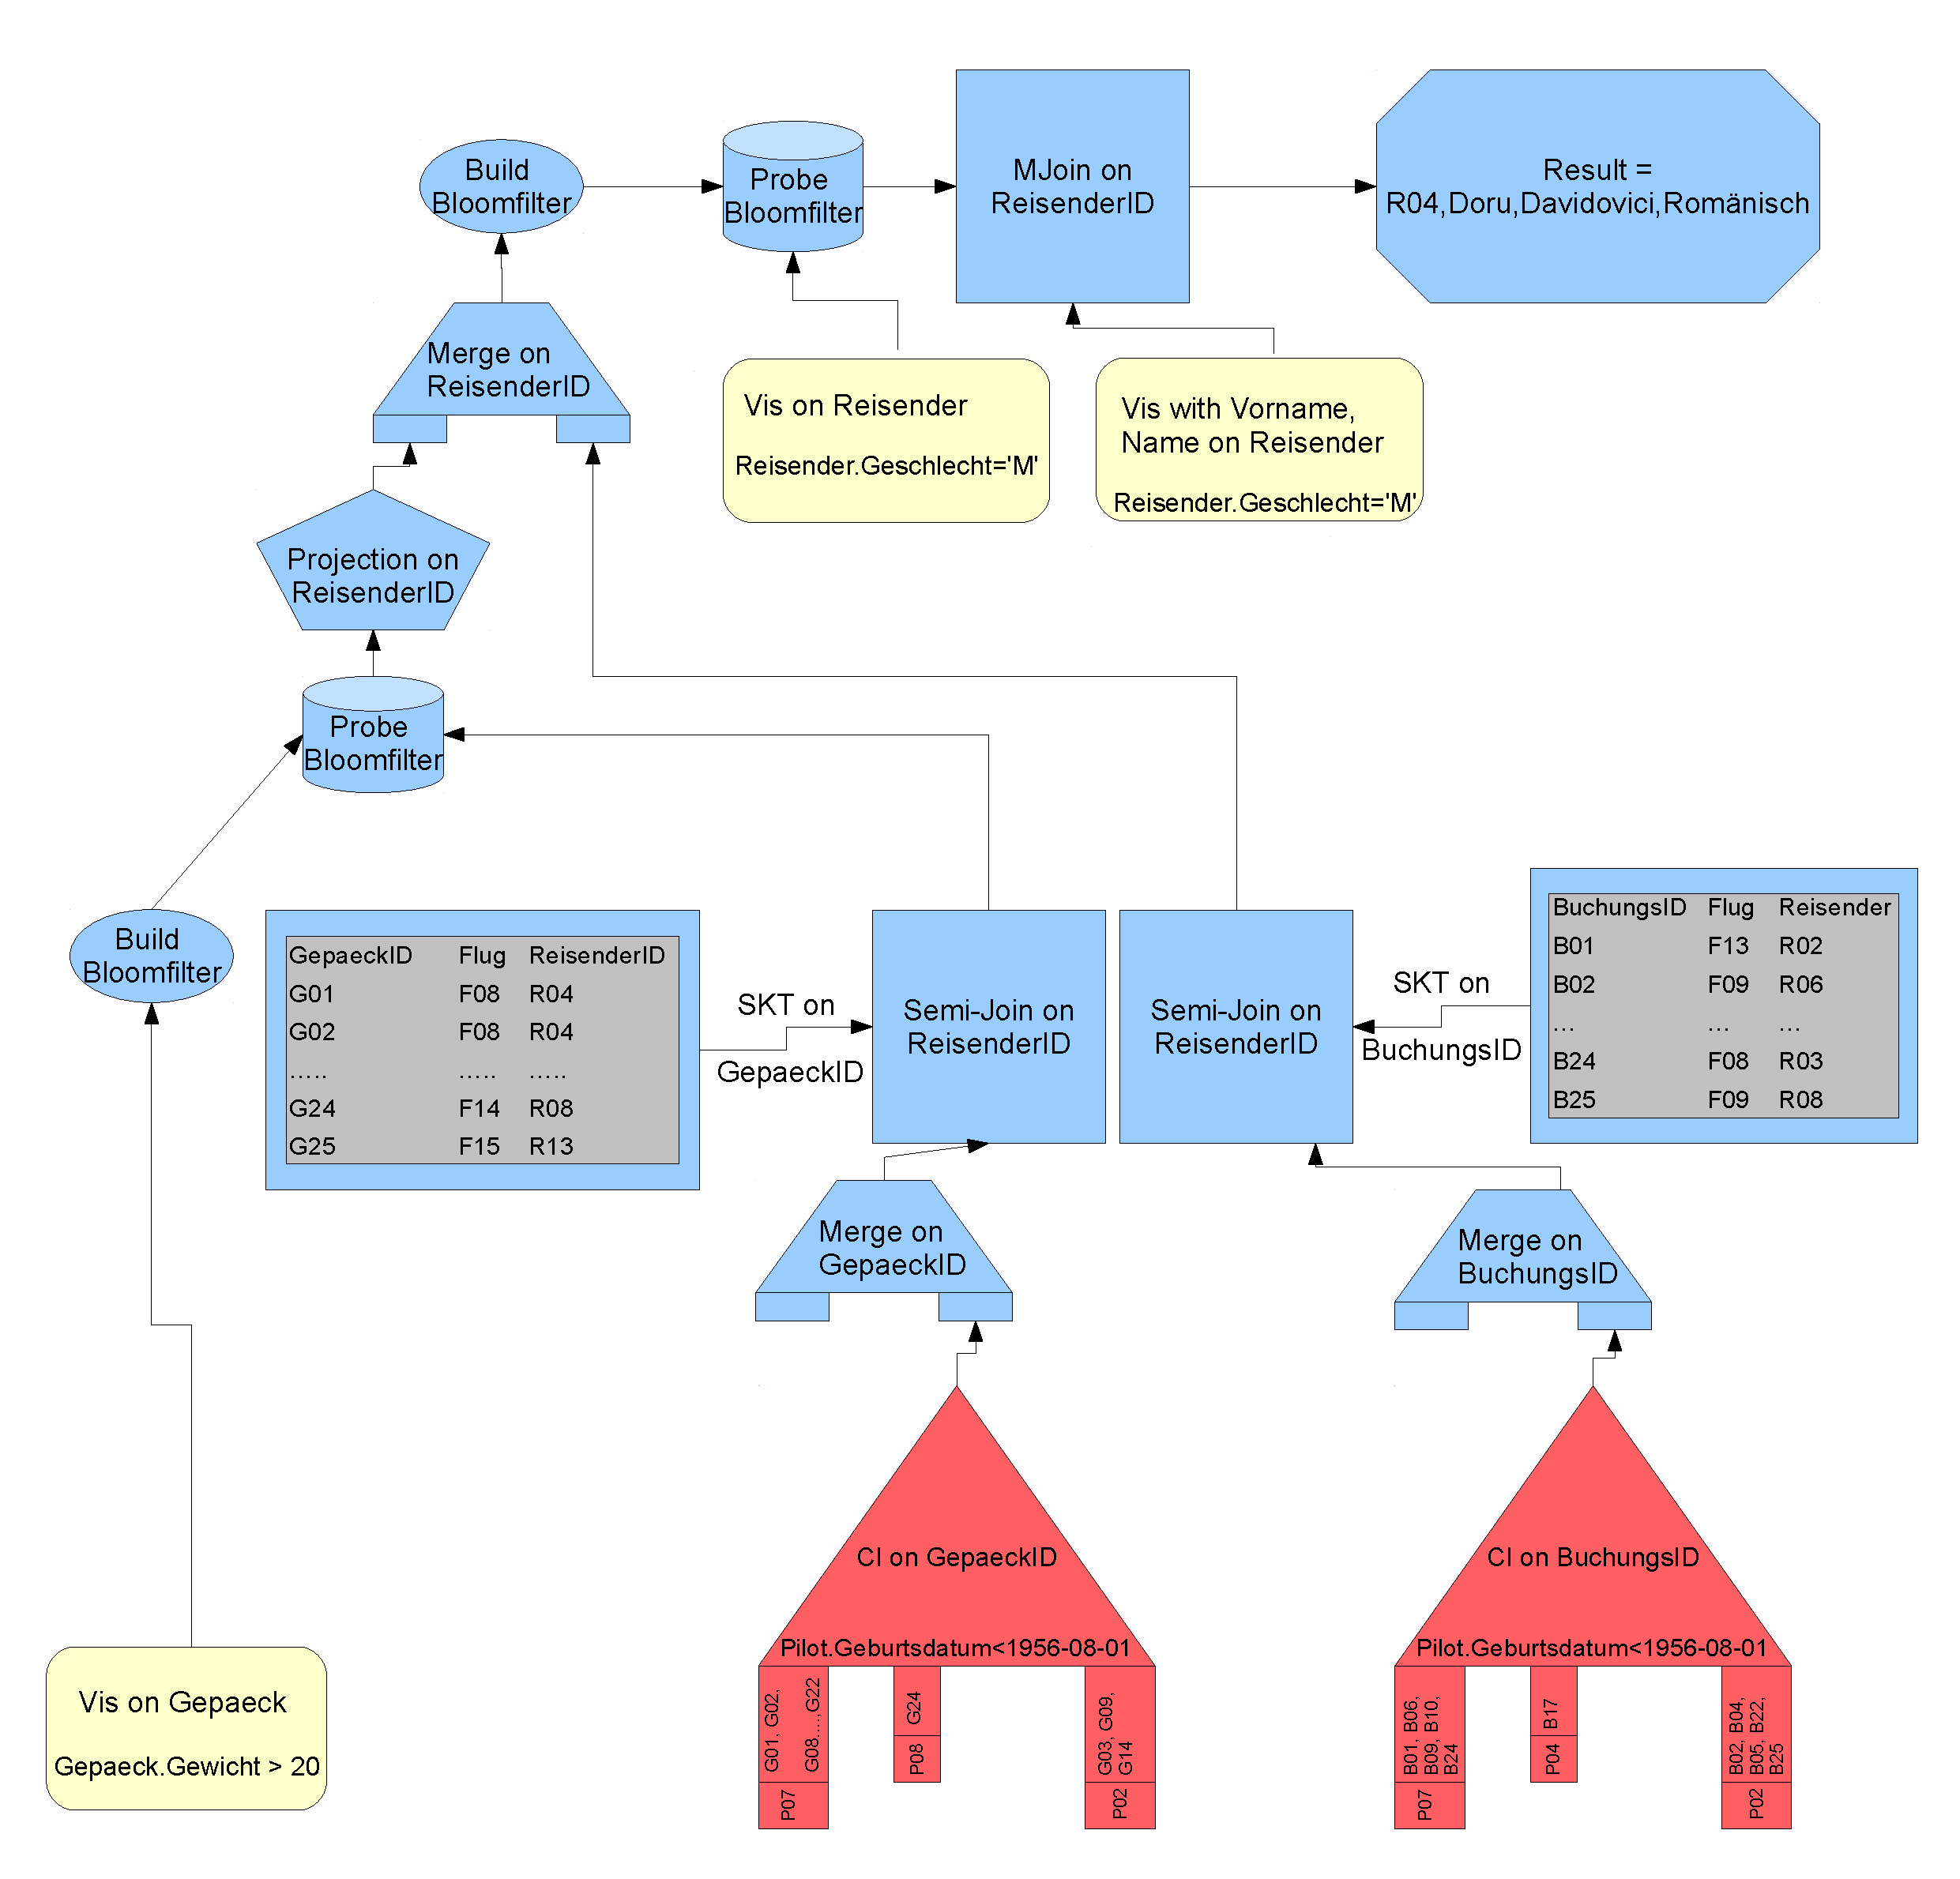
\includegraphics[width=1\textwidth]{img/Post-Filtering.pdf}
  \caption{Post-Filtering QEP}
  \label{fig:post}
\end{figure}

\subsection{Post-Filtering Funktionsaufrufe}
\begin{enumerate}[1]
\item CI(P.Geburtsdatum,<1956-08-01,G.GepaeckID) = \{\{\}, \{G07, G18, G19, G20, G25\}, \{\}, \{\}\}
\item Merge($\bigcup 1$) = \{G07, G18, G19, G20, G22, G23\}
\item SJoin(2,$\text{SKT}_{\text{Gepaeck}}$,$\langle$G.GepaeckID,R.ReisenderID$\rangle$) = \{$\langle$G07,R11$\rangle$, $\langle$G18,R07$\rangle$, $\langle$G19,R04$\rangle$, $\langle$G20,R04$\rangle$, $\langle$G22,R02$\rangle$, $\langle$G23,R01$\rangle$\}
\item Vis(Q,Gepaeck,G.GepaeckID) = \{G06, G12, G13, G16, G18, G19, G20, G22, G23\}
\item BuildBF(4) = BF
\item ProbeBF(BF,3) = \{$\langle$G18,R07$\rangle$, $\langle$G19,R04$\rangle$, $\langle$G20,R04$\rangle$, $\langle$G22,R02$\rangle$, $\langle$G23,R01$\rangle$\}
\item Project(6,R.ReisenderID) = \{R07, R04, R04, R02, R01$\rangle$\}
\item CI(P.Geburtsdatum,<1956-08-01,B.BuchungsID) = \{\{\}, \{B08, B11, B18, B19, B20, B21\}, \{\}, \{\}\}
\item Merge($\bigcup 8$) = \{B08, B11, B18, B19, B20, B21\}
\item SJoin(9,$\text{SKT}_{\text{Buchungen}}$,R.ReisenderID) = \{R07, R03, R13, R05, R04, R11\}
\item Merge($7\cap 10$) = \{R04, R07\}
\item BuildBF(11) = BF
\item Vis(Q,Reisende,R.ReisenderID) = \{R02, R03, R04, R05, R06, R08, R09, R10, R13\}
\item ProbeBF(BF,13) = \{R04\}
\item Vis(Q,Reisende,$\langle$R.ReisenderID,R.Vorname,R.Name$\rangle$) = \{$\langle$R02,Mike,Bannister$\rangle$, \\$\langle$R03,Francis,Chichester$\rangle$, $\langle$R04,Doru,Davidovici$\rangle$, $\langle$R05,Eugene Burton,Ely$\rangle$, $\langle$R06,Charles,Fern$\rangle$, $\langle$R08,Ernst,Heinkel$\rangle$, $\langle$R09,Tony,Jannus$\rangle$, $\langle$R10,Algene,Key$\rangle$, $\langle$R13,Charles,Nungesser$\rangle$\}
\item MJoin(15,14,$\langle$R.ReisenderID,R.Staatsbuergerschaft$\rangle$,11) = \{$\langle$R04,Doru,Davidovici,Rom�nisch$\rangle$\}
\end{enumerate}
